\pdfoutput=1
\documentclass[twocolumn]{aastex61}
%%\documentclass[]{emulateapj}

%Accepted/received/... %%

\received{xxx}
\revised{yyy}
\accepted{zzz}

%% Command to document which AAS Journal the manuscript was submitted to.
\submitjournal{AAS Journals}

%% Short title/authors

\shorttitle{Tidal Torques in Stellar Binaries}
\shortauthors{Fleming et al.}

%% Begin document, title, packages %%
\usepackage{hyperref}
\usepackage{xspace}
\usepackage{graphicx}
\usepackage{amsmath}
\usepackage[caption=false]{subfig}

%% Custom commands
\def\mearth{{\rm\,M_\oplus}}
\def\rearth{{\rm\,R_\oplus}}
\def\msun{{\rm\,M_\odot}}
\def\rsun{{\rm\,R_\odot}}
\def\lsun{{\rm\,L_\odot}}
\def\gsim{~\rlap{$>$}{\lower 1.0ex\hbox{$\sim$}}}
\def\lsim{~\rlap{$<$}{\lower 1.0ex\hbox{$\sim$}}}

\newcommand{\vplanet}[0]{\texttt{VPLanet}\xspace}
\newcommand{\eqtide}[0]{\texttt{EQTIDE}\xspace}
\newcommand{\stellar}[0]{\texttt{STELLAR}\xspace}
\newcommand{\kepler}[0]{\textit{Kepler}\xspace}


%% Begin doc %%

\begin{document}

\title{Rotation Periods in Low-Mass Binary Stars: The Impact of Tidal Torques and Magnetic Braking}

%% AUTHORS %%

%%\correspondingauthor{David P. Fleming}
%%\email{dflemin3@uw.edu}

%%\author[0000-0001-9293-4043]{David P. Fleming}
\author{David P. Fleming}
\affil{Astronomy Department, University of Washington \\
Box 951580, Seattle, WA 98195}

\author{Rory Barnes}
\affiliation{Astronomy Department, University of Washington \\
Box 951580, Seattle, WA 98195}

\author{James R. A. Davenport}
\affiliation{Astronomy Department, University of Washington \\
Box 951580, Seattle, WA 98195}

\author{Rodrigo Luger}
\affiliation{Center for Computational Astrophysics, Flatiron Institute \\
New York, NY 10010}

%% ABSTRACT %%

\begin{abstract}

Stellar rotation period (P$_{rot}$) studies have produced numerous insights into the angular momentum evolution of low-mass stars, but previous investigations have focused on single stars even though roughly half of Sun-like stars are in stellar binaries. Here, we examine how tidal torques, stellar evolution, and magnetic braking shape the P$_{rot}$ evolution of low-mass stellar binaries by performing Monte Carlo simulations of coupled stellar-tidal evolution. We find that tides can modify stellar rotations in binaries with orbital periods (P$_{orb}$) up to 100 days.  At short P$_{orb}$, many stellar binaries tidally-lock into synchronous rotation, naturally producing a population of fast rotators (P$_{rot} < 10$ d) across all stellar masses as is observed in the \textit{Kepler} field, a feature that cannot be reproduced by single-star-only models of magnetic braking.  Many binaries with longer P$_{orb}$ can tidally-lock, fixing the stellar P$_{rot}$ to the binary P$_{orb}$, causing P$_{rot}$ to not be a valid proxy for age in all cases, i.e. gyrochronology methods must be applied carefully. We compare our model predictions with \kepler eclipsing binary (EB) rotation periods and find that our predictions are in excellent agreement with observations, with the ``Constant Time Lag" equilibrium tidal best matching observations.  We show that even for short P$_{orb}$ binaries, tidal torques can balance magnetic braking, producing a population of subsynchronous rotators similar what \citet{Lurie2017} observed in their sample of \kepler EBs. By comparing observations of \kepler EBs with our simulations, we constrain low-mass stellar tidal time lags to $\tau = 0.19^{+0.43}_{-0.16}$ s.

\end{abstract}

%% KEYWORDS %%

\keywords{binaries: close}

%% INTRO %%

\section{Introduction} \label{sec:intro}

Angular momentum evolution in low-mass (M$\lsim 1$ M$_{\odot}$) short-period (P$_{orb} \lsim 10$ d) stellar binaries is dominated by tides.  Tidal torques drive secular changes in the binary orbit and stellar spins, eventually circularizing the orbit and synchronizing the stellar spins in the long-term \citep{Counselman1973}. Orbital circularization is ubiquitous in short-period binaries, owing to the tidal torque's strong semi-major axis dependence, with both theoretical \citep[e.g.][]{Zahn1989} and observational \citep[e.g.][]{Meibom2005,Mazeh2008,Lurie2017} studies finding that most binaries with P$_{orb} \lsim 10$ d are circularized. For short-period binaries, tidal torques work quickly on ${\sim}100$ Myr timescales, as \citet{Zahn1989} finds that the orbit of solar twin binaries circularizes during the stellar pre-main sequence.  Observations by \citet{Meibom2005} support this picture as they find short-period binaries in the ${\sim}150$ Myr old cluster M35 tend to have circular orbits.

Tides impart a significant signature in the long-term angular momentum evolution for binary stars, especially so for the stellar spins. Tidal torques drive stellar spins towards the tidally-locked state in which the stellar P$_{rot}$ is equal to the equilibrium rotation period (P$_{eq}$) predicted by tidal models, with a familiar example of this effect being spin-orbit synchronization where P$_{rot} = $ P$_{eq} = $ P$_{orb}$.  Tidal-locking occurs much earlier than orbital circularization as the tidal-locking timescale is estimated to be $2-3$ orders of magnitude less than the circularization timescale \citep{Zahn1989,Witte2002,Mazeh2008}, and as a result, tidal-locking is expected for binaries with P$_{orb} \lsim$ 20 d \citep[e.g.][]{Meibom2006,Mazeh2008,Zahn2008,Meibom2015}. 

The large sample of $816$ P$_{rot}$ measurements derived using starspot modulations on low-mass \kepler eclipsing binary stars by \citet{Lurie2017} confirm that most short-period binaries are tidally-locked and also show that the tidal torques can influence stellar spins in binaries with P$_{orb}$ up to 45 d. Futhermore, \citet{Lurie2017} shows that a substantial a population of subsynchronous short-period binaries exist in the \kepler field, clustered near P$_{orb}/$P$_{rot}{\sim} 0.9$, in defiance of the expectation of tidal locking.  These findings suggest that that synchronization is not a given for tidally-interacting, short P$_{orb}$  stellar binaries and that impact of tidal effects should be reconsidered for longer P$_{orb}$.  Both the extended \kepler mission \citep[K2,][]{Howell2014} and the Transiting Exoplanet Survey Satellite \citep[TESS, ][]{Ricker2014,Sullivan2015} will detect additional low-mass eclipsing binaries, permitting additional tests for models of stellar angular momentum evolution subject to tidal torques.
 
Understanding angular momentum evolution in low-mass stellar binaries is paramount as P$_{rot}$ distributions measured in clusters \citep[e.g. Praesepe, ][]{Douglas2017} and field stars \citep[e.g. \kepler, ][]{McQuillan2014} are likely contaminated by unresolved binaries, given that roughly half of Sun-like stars are in stellar binaries \citep{Raghavan2010,Duchene2013}, and that binaries are difficult to resolve in photometric surveys. In the \kepler field, for example, \citet{Simonian2018} recently found that most rapid rotators (P$_{rot} \lsim 7.5$ d) are likely non-eclipsing, tidally-synchronized short-period photometric binaries, indicating that tidal torques in binaries can significantly impact observed P${rot}$ distributions.  Even if stellar binaries have not yet tidally-locked, tidal torques modify stellar rotation periods towards the tidally-locked state, away from the long-term spin-down due to magnetic braking predicted for single stars \citep{Dunn1961,Skumanich1972,Barnes2003}, imparting a contaminating signal that is not currently accounted for by modern models. Moreover, any ages inferred from rotation periods of stars in unresolved binaries using gyrochronology, a method that links the long-term spin-down of low-mass stars to their ages, \citep{Skumanich1972,Barnes2003,Barnes2007,Mamajek2008,Barnes2010}, will likely be incorrect owing to the influence of tidal torques. No previous study has quantified this effect.  

Here, we examine angular momentum evolution over the full main sequence lifetimes of low-mass stellar binaries using a realistic treatment of stellar evolution, magnetic braking, and tidal torques. We investigate under what conditions tidal-locking occurs, and how tidal torques influence rotation in stellar binaries as a function of binary P$_{orb}$ and tidal dissipation parameters for two widely-used equilibrium tidal models.  We show how tidal torques can impact stellar rotation in binaries out to P$_{orb} = 100$ d, causing stellar rotation periods to not strongly correlate with age, making the predictions of gyrochronlogy models to fail in such systems.  We describe our model in $\S$~\ref{sec:methods} and our simulation procedure in $\S$~\ref{sec:simulations}.  We discuss how our model impacts rotation period distributions and the implication for gyrochronology methods in $\S$~\ref{sec:gyro}, apply our model to the \kepler field in $\S$~\ref{sec:kepler}, and discuss our results' implications in $\S$~\ref{sec:discussion}.

%% SECTION : Methods %%

\section{Methods} \label{sec:methods}

We simulate coupled stellar-tidal evolution for stellar binaries using an improved version of the coupled stellar-tidal evolution model presented in \citet{Fleming2018}.  We implement our model in the open-source code VPLanet\footnote{VPLanet is publicly available
at \href{https://github.com/VirtualPlanetaryLaboratory/vplanet}{{https://github.com/VirtualPlanetaryLaboratory/vplanet}}.} \citep[][Barnes et al., in prep]{Barnes2016,vplanet2018}.  We integrate all model equations (see $\S$~\ref{sec:methods:stellar} and $\S$~\ref{sec:methods:eqtide}) using using the $4^{th}$ order Runge-Kutta scheme with adaptive timestepping described in \citet{Fleming2018}.  

\subsection{Stellar Evolution} \label{sec:methods:stellar}

We improve upon the stellar evolution model used in \citet{Fleming2018}, \stellar, by tracking the evolution of both the stellar radius of gyration, $r_g$, and radius, $R$, using a bicubic interpolation over mass and time of the \citet{Baraffe2015} stellar evolution models. We model the long-term stellar spin-down due to magnetic braking using the model derived in \citet{Matt2015} since it has been shown to successfully model the spin-down of low-mass stars across many ages in both the Praesepe cluster and in the \kepler field. We model the net change in the stellar rotation rate due to stellar evolution and magnetic braking via the following equation 
\begin{equation} \label{eqn:stellar_rot_rate_dt}
\dot{\omega} = \frac{\dot{J}_{mb}}{I} - \frac{2 \dot{R} \omega}{R} - \frac{2 \dot{r_g} \omega}{r_g}
\end{equation}
where the moment of inertia $I = M r_g^2 R^2$, $\dot{J}_{mb}$ is the angular momentum loss due to magnetic braking, and the time derivatives of the stellar $R$ and $r_g$ are computed numerically using our interpolation of the \citet{Baraffe2015} stellar evolution grids.  

\subsubsection{Example Stellar Evolution} \label{sec:methods:stellarExample}

In Fig.~\ref{fig:stellarExample}, we plot the evolution of $R$, $r_g$, and P$_{rot}$ for 0.2 M$_{\odot}$, 0.7 M$_{\odot}$, and 1 M$_{\odot}$ mass stars, representing an M, K , and G dwarf, respectively, computed according to our stellar evolution model, \stellar. We assume all stars have an initial P$_{rot} = 1$ d and have an initial age of 5 Myr. All stars' radii contract along the pre-main sequence, spinning the stars up (right panel). Once the stars reach the main sequence, their structure changes slowly, allowing magnetic braking to dominate the stellar angular momentum evolution, significantly spinning-down the stars over long timescales. The $r_g$ evolution noticably differs between the stars as the M dwarf's (green) $r_g$ varies little as it remains full convective, while the K and G dwarf grow a radiative core while on the pre-main sequence, decreasing $r_g$ until both reach the main sequence.

\begin{figure*}[ht]
	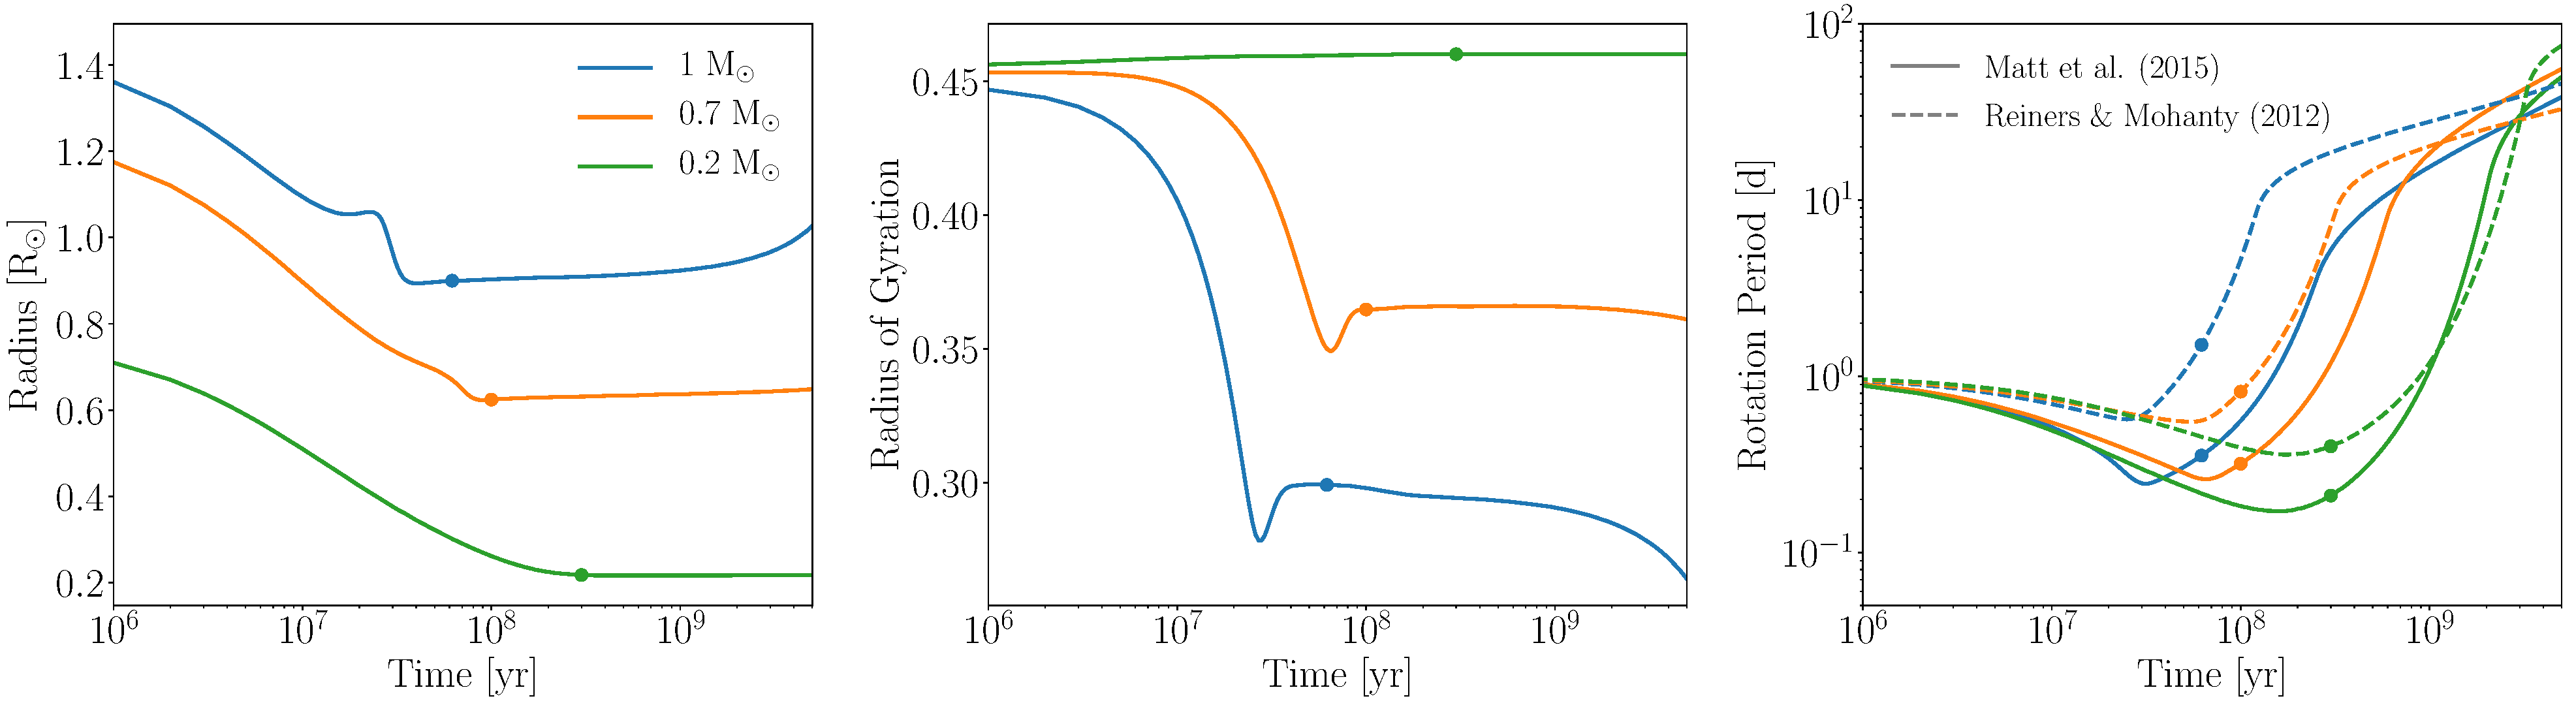
\includegraphics[width=\textwidth]{../Plots/stellarExample.pdf}
   \caption{Stellar $R$ (left), $r_g$ (middle), and P$_{rot}$ (right) evolution for 0.2 M$_{\odot}$ (M, green), 0.7 M$_{\odot}$ (K, orange), and 1 M$_{\odot}$ (G, blue) mass stars computed according to \stellar, our interpolation of the \citet{Baraffe2015} stellar evolution models ($\S$~\ref{sec:methods:stellar}) combined with the \citet{Matt2015} magnetic braking law. Each dot denotes the approximate time when each star reaches the main sequence.}%
    \label{fig:stellarExample}%
\end{figure*}

\subsection{Tidal Evolution} \label{sec:methods:eqtide}

 Equilibrium tidal models, first introduced by \citep{Darwin1880}, track the secular evolution of an orbiter's semi-major axis, $a$, eccentricity, $e$, and the rotation rates, $\omega$, and obliquities $\psi$, of the both gravitating bodies due to tidal torques. Equilibrium tidal models assume that tidally-interacting bodies raise tidal bulges on their companions that remain offset from the line connecting the both bodies' centers of mass due to friction within each body.  The tidal bulges cause torques that drive the exchange of angular momentum between the orbit and both bodies' spins. Equilibrium tidal models are linear since they assume that the tidal waves that comprise the tidal bulge raised on a body are uncoupled. Under these assumptions, the tidal evolution is analogous to a driven, damped harmonic oscillator \citep{Greenberg2009}. For stars, equilibrium tidal models assume that tidal forces dissipate energy in convective regions via viscous turbulence \citep[see][]{Zahn2008}, corresponding to tidal dissipation in the outer convective layers of low-mass stars. We refer the reader to \citet{Barnes2017} for an in-depth discussion of the assumptions and limitations of equilibrium tidal models.  Although simple, equilibrium tidal models have been used to robustly model the secular orbital and rotation evolution of both Solar System bodies and exoplanets \citep[e.g.][]{Goldreich1966,Jackson2009,Leconte2010,Heller2011,Barnes2013,Barnes2017} and stellar binaries \citep[e.g.][]{Zahn1989,Zahn2008,Khaliullin2011,Repetto2014,Fleming2018}. Here, we consider two equilibrium tidal models to study the secular spin-orbital evolution of low-mass stellar binaries.  

\subsubsection{Constant Phase Lag Model}

The ``Constant Phase Lag" (CPL) \citep[][]{FerrazMello2008,Heller2011} equilibrium tidal model assumes that the tidal torque on one body due to its companion arises from a linear combination of several discrete, uncoupled tidal bulges, each with their own associated frequency, that maintain a fixed phase with respect to the line connecting the two stars' centers of mass. We use the \eqtide implementation of the CPL model in VPLanet following the derivation of \citet{FerrazMello2008}.  The equations that govern the secular change in $e$ and $a$ are as follows:

\begin{equation} \label{eqn:cpl:e}
\frac{de}{dt} = -\frac{ae}{8 G m_1 m_2} \sum_{i=1}^2 Z_{i,\mathrm{CPL}} \left( 2 \varepsilon_{0,i} - \frac{49}{2} \varepsilon_{1,i} + \frac{1}{2} \varepsilon_{2,i} + 3 \varepsilon_{5,i} \right)
\end{equation}
\begin{equation} \label{eqn:cpl:a}
\frac{da}{dt} = \sum_{i=1}^2 \frac{da_i}{dt}
\end{equation}
where if the $i^{th}$ body is tidally-locked in a synchronous orbit,
\begin{equation} \label{eqn:cpl:dadt_locked}
\frac{da_{i,sync}}{dt} = -\frac{a^2}{G m_1 m_2} Z_{i,\mathrm{CPL}} \left( 7 e^2 + \sin^2 (\psi_i) \right) \varepsilon_{2,i},
\end{equation}
otherwise
\begin{equation}
\begin{split}
\frac{da_i}{dt} & = \frac{a^2}{4 G m_1 m_2} Z_{i,\mathrm{CPL}} \left( 4 \varepsilon_{0,i} + e^2 \left[ -20 \varepsilon_{0,i} + \frac{147}{2} \varepsilon_{1,i} \right. \right. \\
&  + \left. \left. \frac{1}{2} \varepsilon_{2,i} - 3 \varepsilon_{5,i} \right] - 4 \sin^2 (\psi_i) \left[ \varepsilon_{0,i} - \varepsilon_{8,i} \right] \right).
\end{split}
\end{equation}
The CPL equations for $\psi$ and $\omega$ evolution are
\begin{equation} \label{eqn:cpl:psi}
\frac{d\psi_i}{dt} = \frac{Z_{i,\mathrm{CPL}} \sin(\psi_i)}{4 m_i r_{g,i}^2 R_i^2 n \omega_i} \left( [1-\xi_i] \varepsilon_{0,i} + [1+\xi_i](\varepsilon_{8,i} - \varepsilon_{9,i}) \right)
\end{equation}
\begin{equation} \label{eqn:cpl:omega}
\begin{split}
\frac{d\omega_i}{dt}& = -\frac{Z_{i,\mathrm{CPL}}}{8m_i r_{g,i}^2 R_i^2 n} \left(4 \varepsilon_{0,i} + e^2\left[-20\varepsilon_{0,i} + 49\varepsilon_{1,i} + \varepsilon_{2,i} \right] \right. \\
& \left. + 2 \sin^2(\psi_i) \left[ -2 \varepsilon_{0,i} + \varepsilon_{8,i} + \varepsilon_{9,i} \right] \right)
\end{split}
\end{equation}
where $G$ is Newton's gravitational constant, $n$ is the binary's mean motion, and the index $i$ denotes that $i^{th}$ body. The tidal phase lags signs, $\varepsilon$, for the $i^{th}$ body are given by
\begin{equation} \label{eqn:cpl:eps}
\begin{split}
\varepsilon_{0,i} & = \Sigma(2 \omega_i - 2n) \\
\varepsilon_{1,i} & = \Sigma(2 \omega_i - 3n) \\
\varepsilon_{2,i} & = \Sigma(2 \omega_i - n) \\
\varepsilon_{5,i} & = \Sigma(n) \\
\varepsilon_{8,i} & = \Sigma(\omega_i - 2n) \\
\varepsilon_{9,i} & = \Sigma(\omega_i)
\end{split}
\end{equation}
where the function $\Sigma(x)$ returns $1$ for positive $x$, $-1$ for negative $x$, and $0$ otherwise.

The intermediate variable $Z_{\mathrm{CPL},i}$ is given by
\begin{equation} \label{eqn:cpl:z}
Z_{i,\mathrm{CPL}} = 3 G^2 k_{2,i} M_j^2 (M_i + M_j) \frac{R_i^5}{a^9} \frac{1}{n Q_i}
\end{equation}
where the $j^{th}$ body is the $i^{th}$ body's companion, $k_{2}$ is the body's Love number of degree 2, and $Q$ is the tidal quality factor (``tidal Q"). The tidal Q parameterizes the energy dissipation due to tidal evolution, with lower tidal Qs, i.e. larger phase differences between the tidal bulges, driving more rapid tidal evolution.

The other intermediate variable, $\xi_i$, is defined as
\begin{equation}\label{eqn:cpl:chi}
\xi_i = \frac{r_{\mathrm{g},i}^2 R_i^2 \omega_i a n }{ G M_j}.
\end{equation}

\subsubsection{Constant Time Lag Model}

The ``Constant Time Lag" (CTL) \citep[][]{Hut1981,Leconte2010} equilibrium tidal model assumes a constant time interval between the body's tidal bulge and the passage of the tidally-interacting companion. In this formalism, unlike the CPL model, the CTL model is continuous over a range of tidal wave frequencies.  However if the assumption of linearity is relaxed, i.e. frequencies associate with tidal bulges are allowed to depend on a spin or orbital forcing frequency, then this model is only valid over a small range of frequencies \citep{Greenberg2009}, hence we do not make this assumption and hold the tidal time lag fixed. We use the \eqtide implementation of the CTL model in VPLanet following the derivation of \citet{Leconte2010}.  The equations that govern the secular changes in $e$, $a$, $\omega$, and $\psi$ are as follows:

\begin{equation} \label{eqn:ctl:e}
  \frac{de}{dt} = \frac{11 ae}{2 G M_1 M_2}
  \sum_{i = 1}^2 Z_{\mathrm{CTL},i} \left( \cos(\psi_i) \frac{f_4(e)}{\beta^{10}(e)}  \frac{\omega_i}{n} -\frac{18}{11} \frac{f_3(e)}{\beta^{13}(e)}\right),
\end{equation}

\begin{equation}\label{eqn:ctl:a}
  \frac{da}{dt} \ = \  \frac{2 a^2}{G M_1 M_2}
  \sum\limits_{i = 1}^2 Z_{\mathrm{CTL},i} \left( \cos(\psi_i) \frac{f_2(e)}{\beta^{12}(e)} \frac{\omega_i}{n} - \frac{f_1(e)}{\beta^{15}(e)}\right),
\end{equation}

\begin{equation}\label{eqn:ctl:omega}
  \frac{d\omega_i}{dt} \ = \ \frac{Z_{\mathrm{CTL},i}}{2 M_i r_{g,i}^2 
R_i^2 n} \left( 2 \cos(\psi_i) \frac{f_2(e)}{\beta^{12}(e)} - \left[ 1+\cos^2(\psi)
 \right] \frac{f_5(e)}{\beta^9(e)} 
\frac{\omega_i}{n} \right),  
\end{equation}
and
\begin{equation}\label{eqn:ctl:psi}
  \frac{d\psi_i}{dt} = \frac{Z_{\mathrm{CTL},i} \sin(\psi_i)}{2 M_i r_{g,i}^2 R_i^2 n \omega_i}\left( \left[ \cos(\psi_i) - \frac{\xi_i}{ \beta} \right] \frac{f_5(e)}{\beta^9(e)} \frac{\omega_i}{n} - 2 \frac{f_2(e)}{\beta^{12}(e)} \right).
\end{equation}
where the intermediate variables are given by 
\begin{equation}\label{eqn:ctl:z}
 Z_{i,\mathrm{CTL}} = 3 G^2 k_{2,i} M_j^2 (M_i+M_j) \frac{R_i^5}{a^9} \tau_i ,
\end{equation}
and 
\begin{equation}\label{eqn:ctl:f_e}
\begin{array}{l}
\beta(e) = \sqrt{1-e^2},\\
f_1(e) = 1 + \frac{31}{2} e^2 + \frac{255}{8} e^4 + \frac{185}{16} e^6 + \frac{25}{
64} e^8,\\
f_2(e) = 1 + \frac{15}{2} e^2 + \frac{45}{8} e^4 + \frac{5}{16} e^6,\\
f_3(e) = 1 + \frac{15}{4} e^2 + \frac{15}{8} e^4 + \frac{5}{64} e^6,\\
f_4(e) = 1 + \frac{3}{2} e^2 + \frac{1}{8} e^4,\\
f_5(e) = 1 + 3 e^2 + \frac{3}{8} e^4.
\end{array}
\end{equation}

In both the CPL and CTL model, We assume $k_2 = 0.5$. This choice of $k_2$ does not impact our results as $k_2$ is degenerate with Q in the CPL model, e.g. the $k_2/Q$ scaling in Eq.~(\ref{eqn:cpl:z}), and with $\tau$ in the CTL model, e.g. $k_2 \tau$ scaling in Eq.~(\ref{eqn:ctl:z}), so we instead examine how our results scale with $Q$ and $\tau$.  Any constraints we derive for $Q$ and $\tau$ can trivially be scaled to other values of $k_2$.

\subsubsection{Tidal Locking}

Tidal torques always drive a body towards the tidally-locked state. When a body tidally locks, tidal torques fix P$_{rot}$ to the equilibrium P$_{rot}$, P$_{eq}$.  Typically, tidal locking is understood in the context of a synchronized rotator, e.g. when P$_{rot} = $ P$_{eq} = $ P$_{orb}$. Although spin-orbit synchronization is an expected outcome of tidal evolution \citep{Counselman1973}, in general for tidally-locked bodies on non-circular orbits, both the CPL and CTL model predict pseudosynchronous, or supersynchronous rotation, e.g. Mercury's 3:2 spin-orbit resonance \citep[P$_{rot} = 2/3$ P$_{orb}$,][]{GoldreichPeale1966}.   

The CPL model, owing to its assumption of a finite number of discrete tidal lags, only permits a 1:1 and 3:2 spin-orbit state where, following \citet{Barnes2017}, the CPL P$_{eq}$ is given by
\begin{equation} \label{eqn:cpl:eqPer}
P^{\mathrm{CPL}}_{eq} = 
\begin{cases}
P_{orb} & \text{if } e < \sqrt{1/19}\\
\frac{2}{3}P_{orb} & \text{if } e \geq \sqrt{1/19}.
\end{cases}
\end{equation}
Therefore, the CPL model predicts synchronous rotation for $e \lsim 0.23$, and a supersychronous 3:2 spin-orbit state otherwise for tidally-locked rotators.

The CTL model, however, is continuous over a range of tidal frequencies and therefore predicts a P$_{eq}$ that is a continuous function of both $e$ and $\psi$.  Following \citet{Barnes2017}, we define the CTL P$_{eq}$ by
\begin{equation} \label{eqn:ctl:eqPer}
P^{\mathrm{CTL}}_{eq} = P_{orb} \frac{\beta^3 f_5(e) (1 + \cos^2(\psi))}{2f_2(e) \cos(\psi)}.
\end{equation}
The CTL model predicts that bodies on eccentric orbits tidally-lock into supersyncronous rotation, and only bodies with aligned spins on circular orbits are synchronous rotators. 

Due to the discontinuities in the equilibrium tidal model equations, for example in Eq.~(\ref{eqn:cpl:eps}) when $\omega \approx n$, and due to the inherant discreteness of numerical integrations, numerical solutions for the CPL and CTL models can produce unphysical evolution. We follow \citet{Barnes2013} and \citet{Fleming2018} and fix P$_{rot} = $ P$_{eq}$ according to Eq.~(\ref{eqn:cpl:eqPer}) or Eq.~(\ref{eqn:ctl:eqPer}) for the CPL and CTL models, respectively, when P$_{rot}$ is within $1\%$ of P$_{eq}$.  To ensure that tidal torques dominate over torques due to magnetic braking and stellar evolution, we additionally require that the P$_{rot}$ derivative points towards $P_{eq}$ on both sides of P$_{eq}$, i.e. when the gradient of P$_{rot}$ points towards the tidally-locked state, before fixing P$_{rot} = $ P$_{eq}$. We find that this scheme produces physically and numerically accurate results. 

\subsubsection{Example Tidal Evolution} \label{sec:methods:eqtideExample}

We plot the tidal evolution for $a$, $e$, and $\omega$, ignoring stellar evolution, for a solar-twin binary with an initial P$_{orb} = 10$ d, P$_{rot} = 1$ d, $e = 0.2$ for the CPL model and CTL model, assuming $Q=10^6$ and $\tau = 0.1$ seconds, respectively, in Fig.~\ref{fig:tidalExample}. Both the CPL and CTL model predict the same qualitative evolution: both the binary's $e$ and P$_{orb}$ slightly increasing as tides force the spins toward the tidally-locked state, transfering rotational angular momentum into the orbit in the process.  At late times, both the CPL and CTL drive the binaries towards orbital circularization, with tidal dissipation decreasing P$_{orb}$. The predictions of the CPL and CTL model, differ, however, when the binaries tidally-lock.  Under the CPL model, the binary tidally-locks into a synchronous orbit as $e < \sqrt{1/19}$, e.g. Eq.~(\ref{eqn:cpl:eqPer}), while the CTL model predicts supersyncronous rotation due to the CTL model's equilibrium period eccentricity dependence, e.g. Eq.~(\ref{eqn:ctl:eqPer}).

\begin{figure}
	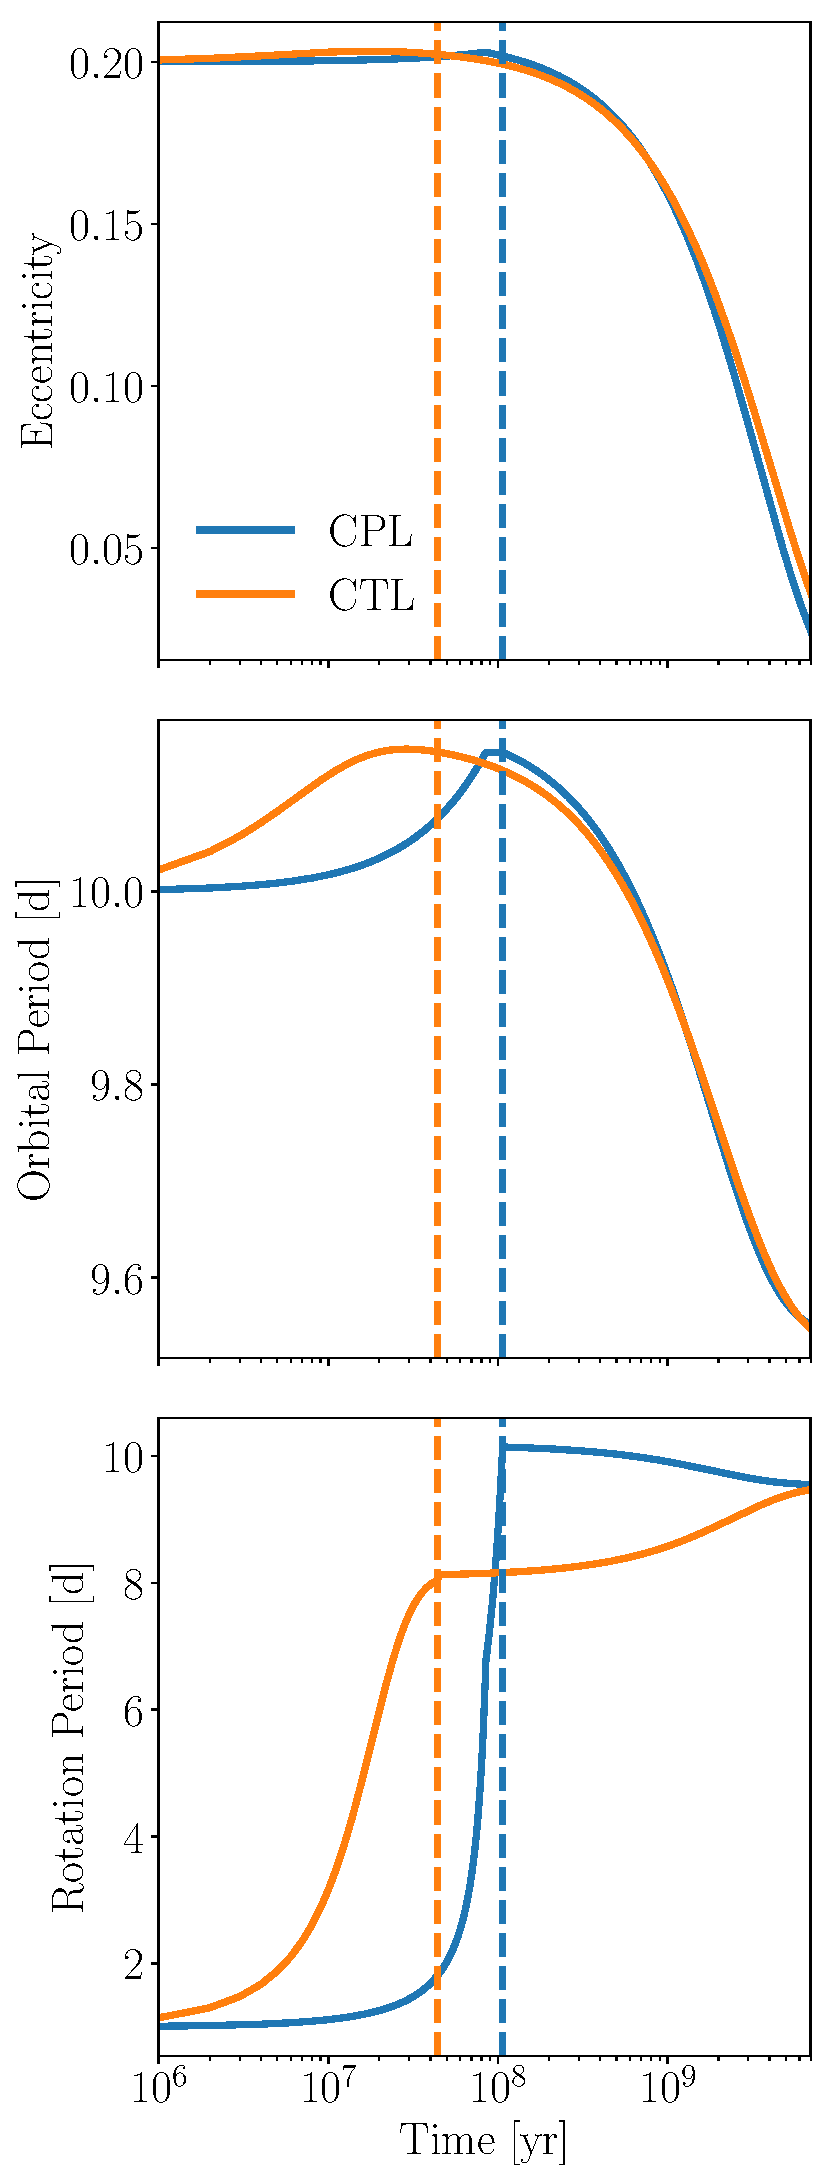
\includegraphics[width=0.4\textwidth]{../Plots/tidalExample.pdf}
   \caption{Tidal evolution of a 1 M$_{\odot} -$ 1 M$_{\odot}$ stellar binary's $e$ (top), P$_{orb}$ (middle) and P$_{rot}$ (bottom) for the CPL (blue) and CTL (orange) model. The blue (CPL) and orange (CTL) vertical dashed lines denote when the stellar binary tidally-locks. Both the CPL and CTL model predict the same qualitative evolution. The rotational evolution differs, however, as under the CPL model, the binary tidally-locks into a synchronous orbit as $e < \sqrt{1/19}$, e.g. Eq.~(\ref{eqn:cpl:eqPer}), while the CTL model predicts supersyncronous rotation due to the CTL model's equilibrium period eccentricity dependence (see Eq.~(\ref{eqn:ctl:eqPer})).}%
    \label{fig:tidalExample}%
\end{figure}

\subsection{Coupled Stellar-Tidal Evolution For Tidally-Locked Systems} \label{sec:coupled}

Following \citet{Fleming2018}, when one or both binary stars are tidally locked, tidal forces prevent magnetic braking from spinning down the tidally-locked star(s), and any angular momentum lost is lost at the expense of the binary orbit, decreasing $a$ as a result \citep{Verbunt1981}.  Below in Eq.~(\ref{eqn:tidal_locked_one}) and Eq.~(\ref{eqn:tidal_locked_two}), we modify the $a$ decay equations due to stellar evolution and magnetic braking in tidally-locked binaries from \citet{Fleming2018}, their Eqs. (18) and (20), to additionally account for $r_g$ evolution when one or both stars tidally-lock, respectively, assuming conservation of angular momentum:
\small
\begin{equation} \label{eqn:tidal_locked_one}
\begin{split}
\dot{a}_{coupled}^{(1)} = \frac{-\dot{J}_{mb} - 2 \omega \left( m_1 r_{g,1}^2 R_1 \dot{R_1} - m_1 r_{g,1} \dot{r}_{g,1} R_1^2 \right)}
{\frac{\mu^2 G M (1-e^2)}{2J_{orb}} - \frac{3 \omega}{2a} m_1 r_{g,1}^2 R_1^2}
\end{split}
\end{equation}
\normalsize
and
\small
\begin{equation} \label{eqn:tidal_locked_two}
\begin{split}
\dot{a}_{coupled}^{(2)} = \frac{-\dot{J}_{mb} - 2 \omega \left( \sum_{i=1}^{2} m_i r_{g,i}^2 R_i \dot{R_i} + m_i r_{g,i} \dot{r}_{g,i} R_i^2 \right)}
{\frac{\mu^2 G M (1-e^2)}{2J_{orb}} - \frac{3 \omega}{2a} \left( m_1 r_{g,1}^2 R_1^2 + m_2 r_{g,2}^2 R_2^2 \right)}.
\end{split}
\end{equation}
\normalsize
where $J_{orb}$ is the orbital angular momentum.

%% SECTION: Simulations + Initial conditions %%
\section{Simulations} \label{sec:simulations}

We examine stellar angular momentum evolution in low-mass binaries by performing a Monte Carlo study of two sets of 10,000 stellar binaries, one modeled using the CPL model and the other using the CTL formalism.  We simulate both stars' spin evolution but mainly consider the P$_{rot}$ evolution for the primary, i.e. more massive star in binaries, as it is observationally easier to measure a P$_{rot}$ on the more massive, and hence brighter, star \citep[e.g.][]{Meibom2006,Lurie2017}. For each simulation, we sample the primary's mass uniformly over $[0.1, 1]$ M$_{\odot}$. Following \citet{Matt2015}, we uniformly sample the log$_{10}$ of P$_{rot}$ over [$0.8,15$] days, a distribution that approximates the P$_{rot}$ distribution of young stars in the ${\sim}2$ Myr old ONC.  We compute the secondary star's mass by uniformly sampling the mass ratio over [$0.1, 1$] following observations of mass ratios in low-mass binaries \citep{Raghavan2010,Moe2018}. Given the inherent uncertainty in and complexity of the formation of binaries \citep[e.g.][]{Bonnell1994,Bate2000,Bate2002,Moe2018} and the potential for dynamical processing via tides or stellar close encounters \citep[e.g.][]{Mardling2001,Hurley2002,Ivanova2005,Meibom2005}, we take an agnostic approach to the initial orbital configuration by uniformly randomly sampling the initial eccentricity ($e$) over [$0.0,0.3$] and uniformly sampling the initial P$_{orb}$ over [$3,100$] d. Although the CTL model is applicable for $e > 0.3$, the CPL model is not, so we restrict $e \leq 0.3$ to allow us to compare both models. We do not consider P$_{orb} < 3$ d as these binaries are likely to have a tertiary companion \citep{Tokovinin2006} which can significantly impact the inner binaries' dynamical evolution \citep[e.g.][]{Munoz2015,Martin2015b,Hamers2016,Moe2018}. 

Values for stellar tidal $Q$s and $\tau$s for low-mass stars are highly uncertain, likely depend on complex viscous evolution within the stars \citep{Ogilvie2007}, can differ for stars of the same spectral class \citep{Barker2009}, and can vary as a function of stellar age \citep{Bolmont2016}, likely due to low-mass star's evolving convective regions where the tidal dissipation predominantly occurs \citep{Zahn2008}. Typical values of $Q$ and $\tau$ for Sun-like stars are estimated to be of order $Q \approx 10^6$ and $\tau \approx 0.1$ s, respectfully \citep[e.g.][]{Meibom2005,Ogilvie2007,Jackson2009}, however a wide range of values exist in the literature.  Therefore, we consider a wide range of tidal parameters by sampling stellar tidal Qs loguniformly over $[10^4,10^7]$ and $\tau$ loguniformly over $[10^{-2},1]$ s.  All stars have an initial age of 5 Myr unless stated otherwise as by this time, the gaseous protoplanterary circumbinary disk that can impart significant dynamical changes in the system \citep[e.g.][]{Fleming2017} would likely have dissipated \citep{Haisch2001}.

We also perform a smaller subset of simulations to illustrate the behaviour of our coupled model and describe their initial conditions as we introduce them. All code used to run simulations and generate figures is available online\footnote{\href{https://github.com/dflemin3/sync}{https://github.com/dflemin3/sync}.} with accompanying descriptions and documentation.

%% SECTION: RESULTS %%

\section{Results} \label{sec:results}

\subsection{The Weak Tidal Torque Regime} \label{sec:eq}

Here we examine the P$_{rot}$ evolution of 1 M$_{\odot} - 1$ M$_{\odot}$ binaries on initially circular orbits with a focus on systems with weak tidal torques, i.e. long P$_{orb}$ and large $Q$ or small $\tau$, to examine the boundry between evolution dominated by tides or magnetic braking.  In Fig.~\ref{fig:eqPer}, we plot the evolution of P$_{rot}$, normalized by P$_{eq}$, and its time derivative for P$_{orb} \in [5,60]$ d modeled using both the CPL (solid line, $Q=10^6$) and CTL (dashed line, $\tau = 0.1$ s) formalisms. Both models predict that binaries with P$_{orb} < 10$ d will tidally-lock within 100 Myr, in agreement with observations \citep{Meibom2005} and previous theoretical work \citep{Zahn1989}. The CPL model predicts that each binary tidally-locks, even out to P$_{orb} = 60$ d, indicating that tidal locking is not necessarily to short P$_{orb}$ systems. 

\begin{figure*}
	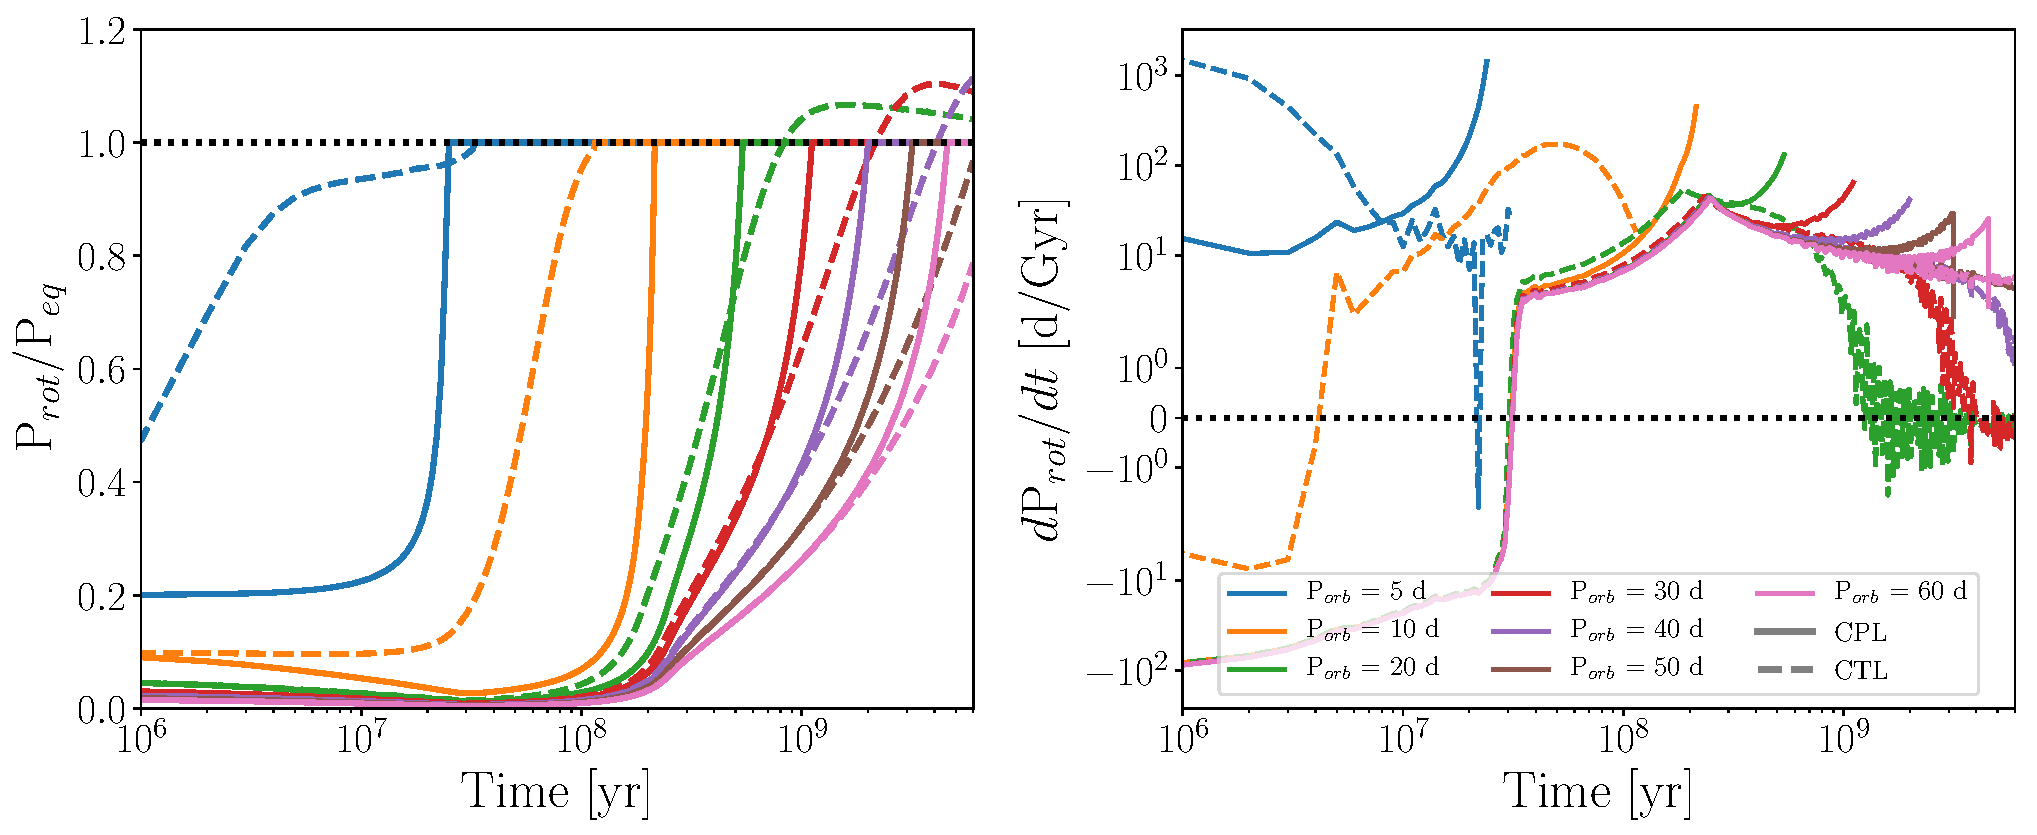
\includegraphics[width=\textwidth]{../Plots/eqPerTwoPanel.pdf}
   \caption{Evolution of stellar P$_{rot}$, normalized by P$_{eq}$ (see Eqn.~(\ref{eqn:cpl:eqPer}) and Eqn.~(\ref{eqn:ctl:eqPer}), for initial circular binary orbits according to the CPL (solid) and CTL (dashed) models with $Q = 10^6$ and $\tau = 0.1$ s, respectively. Left: P$_{rot}/$P$_{eq}$ for stars with P$_{orb}$ ranging from 5 d to 60 d. The black dotted line indicates that tidally-locked state where P$_{rot} = $ P$_{eq}$.  Right: Net P$_{rot}$ derivative due to stellar evolution, tidal torques, and magnetic braking.  We truncate each curve when the binary tidally-locks. For P$_{orb} \leq 10$ d, both the CPL and CTL models predict that the binaries lock into synchronous rotation.  For all P$_{orb}$, the CPL models tidally-lock into synchronous rotation whereas the CTL model predicts subsynchronous (P$_{rot} > $ P$_{eq}$) rotation that persists for Gyrs.}%
    \label{fig:eqPer}%
\end{figure*}

% caption extra: 
%In the CTL cases, magnetic braking overpowers tidal torques, spinning down the stars, preventing tidal-locking.  Tidal torques eventually overpower magnetic braking for long P$_{rot}$ \citep{Kawaler1988,Matt2015}, slowly driving the stellar rotation back towards the tidally-locked state. 
% Initially, all systems spin-up due to stellar radius contraction. Once the stars reach the main sequence at ${\sim} 60$ Myr, tidal torques and magnetic braking combine to spin down the stars towards the tidally-locked state. For many CTL models, $\dot{\mathrm{P}}_{rot} > 0$ as magnetic braking overpowers tidal torques causing sustained subsynchronous rotation.  After spinning down to long P$_{rot}$, magnetic braking weakens, allowing tidal torques to sheppard P$_{rot}$ towards P$_{eq}$ as the P$_{rot}$ derivatives stay near 0, but with a slight negative value.

The CTL model, however, predicts that for P$_{orb} \gsim 10$ d, magnetic braking overpowers weak tidal torques, spinning down the stars past the tidally-locked state. Magnetic braking pushes P$_{rot}/$P$_{eq} > 1$ with the maximum value set by the torque balance between tidal torques and magnetic braking. The maximum values grows for longer P$_{orb}$ since tides weaken with increasing binary separation, e.g. Eqn.~(\ref{eqn:ctl:z}), allowing magnetic braking to dominate the spin evolution.  After reaching the maximum, however, P$_{rot}$ decreases back towards the tidally-locked state in the long-term due to a combination of three simultaneous physical effects.  First, as P$_{rot}$ continue to slow, magnetic braking weakens as its torque scales as $\omega$ or $\omega^3$ \citep{Kawaler1988}, depending on if the stars are in the saturated or unsaturated regime, respectively \citep{Matt2015}.  Second, as P$_{rot}$ slows down further from the tidally-locked state, tidal torques strengthen as they try to force P$_{rot}$ back towards P$_{eq}$ (see Eqn.~(\ref{eqn:ctl:omega}), for example). Third, when P$_{rot} > $ P$_{eq}$, P$_{orb}$ decreases as tides transfer angular momentum from the orbit into stellar rotations, strengthening tidal torques that depend on the binary separation as $a^{-6}$.  These effects combine to shift the balance of power from magnetic braking-controlled stellar spin down to tidal torques spinning-up stars, shepparing them towards P$_{eq}$ in the long term. 

We can see this process unfold in the right panel of Fig.~\ref{fig:eqPer} where we plot the total P$_{rot}$ time derivative due to stellar evolution, magnetic braking, and tidal torques. Early on, $\dot{\mathrm{P}}_{rot} < 0$ as stars contract along the pre-main sequence until about 100 Myr. After $R$ contraction, $\dot{\mathrm{P}}_{rot} > 0$ as tides and magnetic braking combine to spin down stars towards the tidally-locked state. For the CTL models with P$_{orb} > 10$ d, $\dot{\mathrm{P}}_{rot} > 0$, but $\ddot{\mathrm{P}}_{rot} < 0$ as the three processes described above gradually strengthen tidal torques relative to magnetic braking.  In the long-run, tidal torques overpower magnetic braking, with a slightly negative P$_{rot}$ derivative, slowly driving P$_{rot}$ towards P$_{eq}$ (see the P$_{orb} = 20, 40$ d cases in Fig.~\ref{fig:eqPer}). This slowly shifting torque balance produces a population of subsynchronous rotators with P$_{rot} \gsim $ P$_{eq}$ that can persist for Gyrs.  

\begin{figure}
	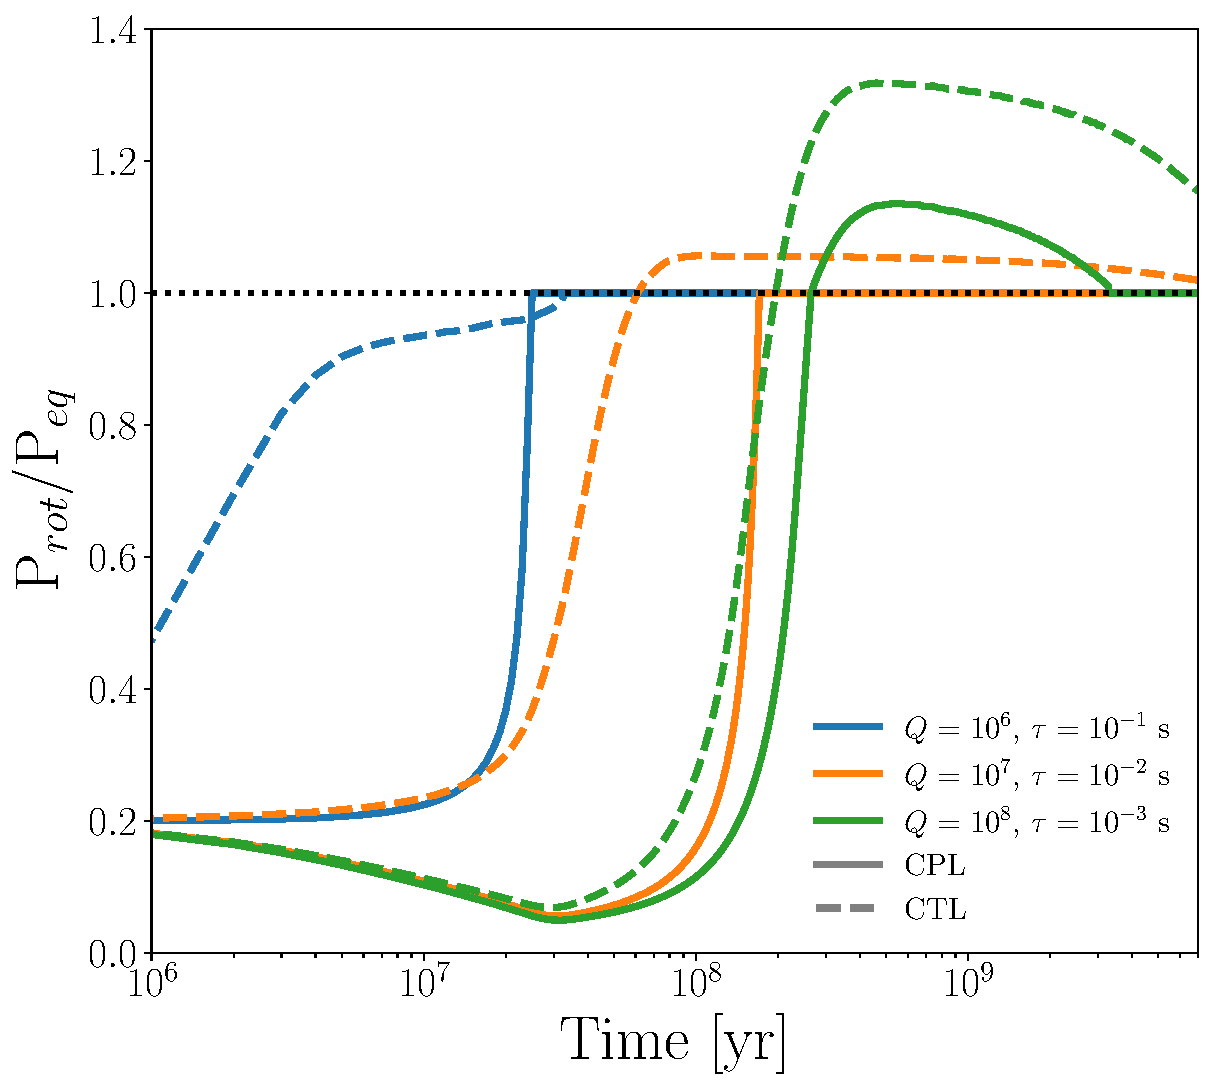
\includegraphics[width=0.45\textwidth]{../Plots/eqPerShortPorb.pdf}
   \caption{Evolution of stellar P$_{rot}$, normalized by P$_{eq}$ (see Eqn.~(\ref{eqn:cpl:eqPer}) and Eqn.~(\ref{eqn:ctl:eqPer}), for initial circular binary orbits with initial P$_{orb} = 5$ d according to the CPL (solid) and CTL (dashed) models for several values of $Q$ and $\tau$, respectively. Systems with strong tidal torques ($Q = 10^6$ or $\tau = 0.1$ s) tidally-lock, whereas in systems with weaker tidal torques (larger $Q$ and smaller $\tau$, respectively), magnetic braking initially overpowers tidal torques, spinning down the stars past the tidally-locked state, resulting in subsynchronous rotation. }%
    \label{fig:eqPerShortPorb}%
\end{figure}

% caption extra:
% In the long-term, magnetic braking weakens relative to tidal torques for longer P$_{rot}$, allowing tides to drive the stars back towards the tidally-locked state.

Spin-orbit synchronization should not be assumed for short P$_{orb}$ binaries. In Fig.~\ref{fig:eqPerShortPorb}, we plot the P$_{rot}$ evolution for a P$_{orb} = 5$ d binary for various tidal dissipation parameters and find that subsynchronous rotation occurs in the general case of weak tidal torques, $Q>10^7$ or $\tau < 0.1$ s in these cases, and is not restricted to long P$_{orb}$ binaries.  Moreover, short P$_{orb}$ subsynchronous rotators can eventually tidally-lock via the mechanism described above where tidal torques gradually strengthen relative to magnetic braking. Short P$_{orb}$ subsynchronous binaries exist in nature, such as some \kepler EBs (\citet{Lurie2017}, see $\S$~\ref{sec:kepler} for further discussion), Kepler-47 \citep{Orosz2012} and a Ruprecht 147 eclipsing binary \citep{Torres2018}, suggesting that this theoretical observation is real.  We explore this effect further in $\S$~\ref{sec:subsync} and describe how we can use it to constrain the tidal parameters $Q$ and $\tau$.

\subsection{Influence of P$_{orb}$, $Q$ and $\tau$}

We examine how P$_{rot}$ evolution in stellar binaries depends on P$_{orb}$ and the strength of tidal dissipation, parameterized by $Q$ and $\tau$ for the CPL and CTL models, respectfully, and connect them to observables. In Fig.~\ref{fig:qTauLock}, we bin our simulation results after the full 7 Gyr evolution by P$_{orb}$ and $Q$ or $\tau$ and compute the median P$_{orb}/$P$_{rot}$ in each bin, marginalizing over all other parameters.

Spin-orbit synchronization is the typical outcome for tidally-interacting binaries according to the CPL model, with synchronization occurring for most binaries with P$_{orb} < 10$ d, regardless of $Q$. The strong tidal torques predicted by the CPL model can even tidally-lock binaries out to P$_{orb} \approx 100 $ d for $Q < 10^5$, well beyond the expected limit of 20 d \citep{Meibom2006}.  According to the CTL model, binaries with P$_{orb} < 10$ d typically tidally-lock for $\tau \gsim 0.1$ s, and seldomly tidally-lock for P$_{orb} > 20$ d, regardless of $\tau$.  Both models predict a substantial population of subsynchronous rotators (red regions in Fig.~\ref{fig:qTauLock}, P$_{rot} >$ P$_{orb}$), consistent with magnetic braking dominating weak tidal torques, i.e. stars with large $Q$ or small $\tau$, that form via the mechanism described in $\S$~\ref{sec:eq}, with weaker the tidal torques allowing more subsynchronous rotation.  The population of supersynchronous rotators (blue regions in Fig.~\ref{fig:qTauLock}, P$_{rot} <$ P$_{orb}$) with P$_{orb} > 80$ d does not in general correspond to binaries tidally-locking into supersynchronous rotation, but rather, typically arises from the combination of weak tidal torques and magnetic braking not spinning down stars enough for P$_{rot}$ to be close to the tidally-locked state.  Under both tidal models, there is a population of nearly synchronous rotators near P$_{orb} \approx 60$ d.  This population corresponds to the evolution described in $\S$~\ref{sec:eq} in which magnetic braking initially spins down stars past the tidally-locked state, but in the long-term, tidal torques spin up the stars, shepparding them towards the tidally-locked state.  This process can keep stellar P$_{rot} \gsim$ P$_{eq}$ for several Gyrs or longer, depending on the P$_{orb}$ (see Figs.~\ref{fig:eqPer},\ref{fig:eqPerShortPorb}). 

\begin{figure*}[ht]
	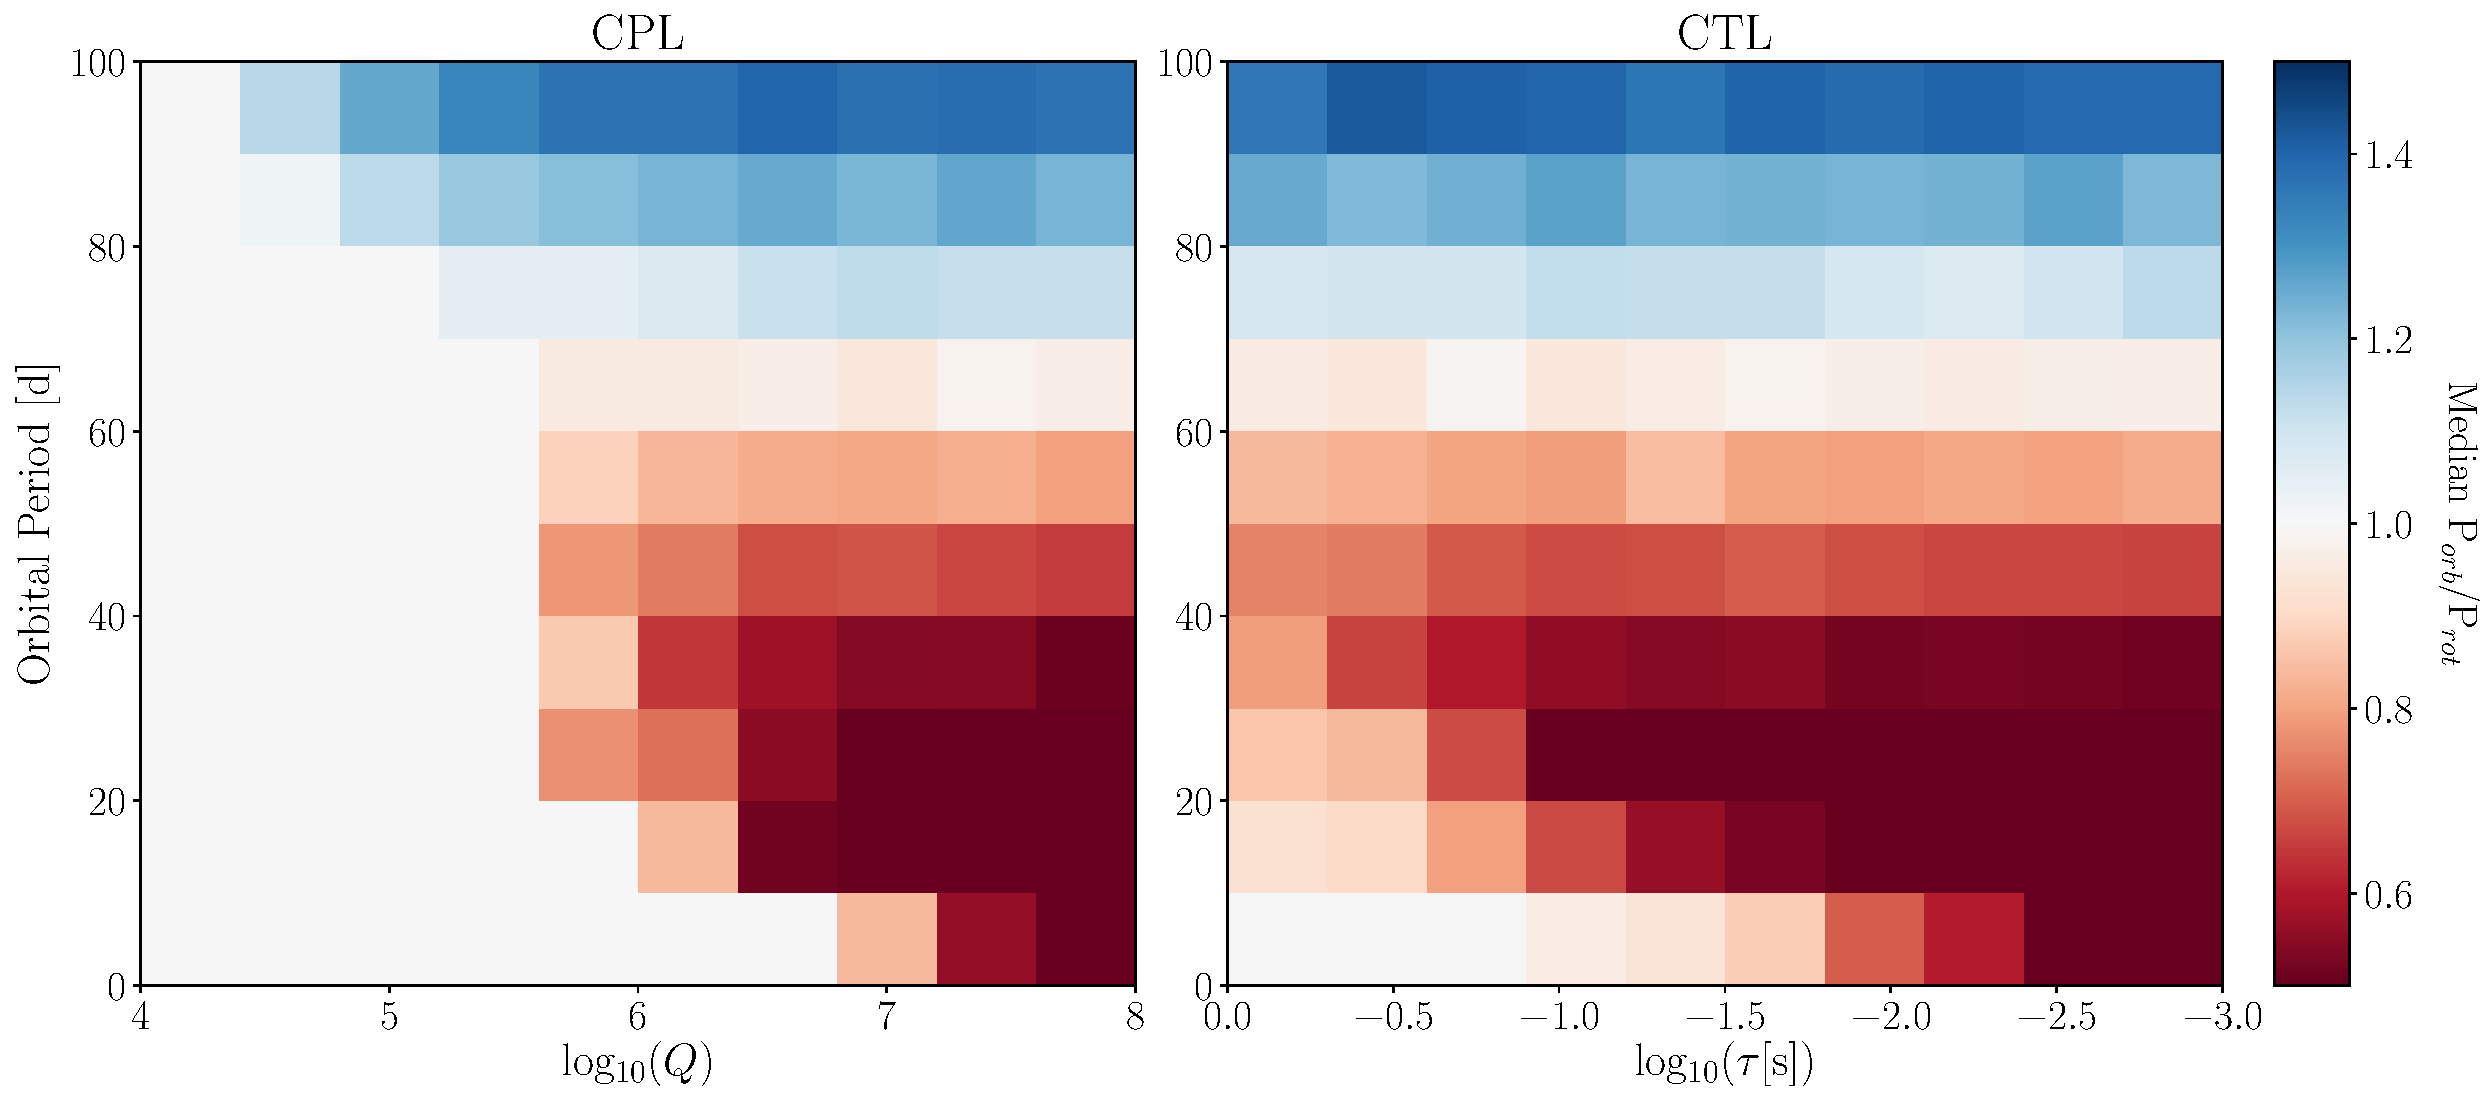
\includegraphics[width=\textwidth]{../Plots/qTauPorbRatioHist.pdf}
   \caption{Median P$_{orb}/$P$_{rot}$ at the end of the simulation according to the CPL (left) and CTL (right) models binned by log$_{10}(Q)$ and log$_{10}(\tau)$, respectively, and P$_{orb}$.  For P$_{orb} < 10$ d, the CPL model predicts that most systems will tidally-lock into synchronous rotation, regardless of $Q$, whereas the CTL model requires $\tau \geq 0.1$ s to tidally-lock.  Both models exhibit supersynchronous rotation (blue regions, P$_{rot} <$ P$_{orb}$) for P$_{orb} > 80$d, that do not in general reflect tidally-locking into a supersynchronous rotation, but rather at long P$_{orb}$, the combination of weak tidal torques and magnetic braking have not spin down the star enough for P$_{rot}$ to be close to P$_{orb}$ after 7 Gyr of evolution. For large $Q$ ($Q > 10^{6.5}$) and small $\tau$ ($\tau < 0.1$ s), weak tidal torques cannot prevent magnetic braking from spinning down stars past the tidally-locked state, producing a population of subsynchronous (red regions, P$_{rot} >$ P$_{orb}$) rotators.}%
    \label{fig:qTauLock}%
\end{figure*}

% caption extra:
% The CPL model predicts that stellar binaries can tidally-lock out to P$_{orb} = 30$ d for most values of $Q$, with some locking all the way up to P$_{orb} = 100$ d for small $Q < 10^5$.  

From Fig.~\ref{fig:qTauLock}, certain rotation states, e.g. synchronous rotation, typically occur in certain regions of parameter space, e.g. where tidal torques are dominant, small $Q$ or large $\tau$. Therefore by measuring P$_{rot}$ and P$_{orb}$ for the primary star in a binary system, one can in principle constrain the strength of the tidal interaction that led to that rotation state. We do so in Fig.~\ref{fig:qmap} and Fig.~\ref{fig:taumap} by binning our simulation results after 7 Gyr of evolution by P$_{orb}$ and P$_{orb}/$P$_{rot}$ and computing the median $Q$ and $\tau$, and the $16\%$, and $84\%$ percentiles, in each bin.

\begin{figure}
	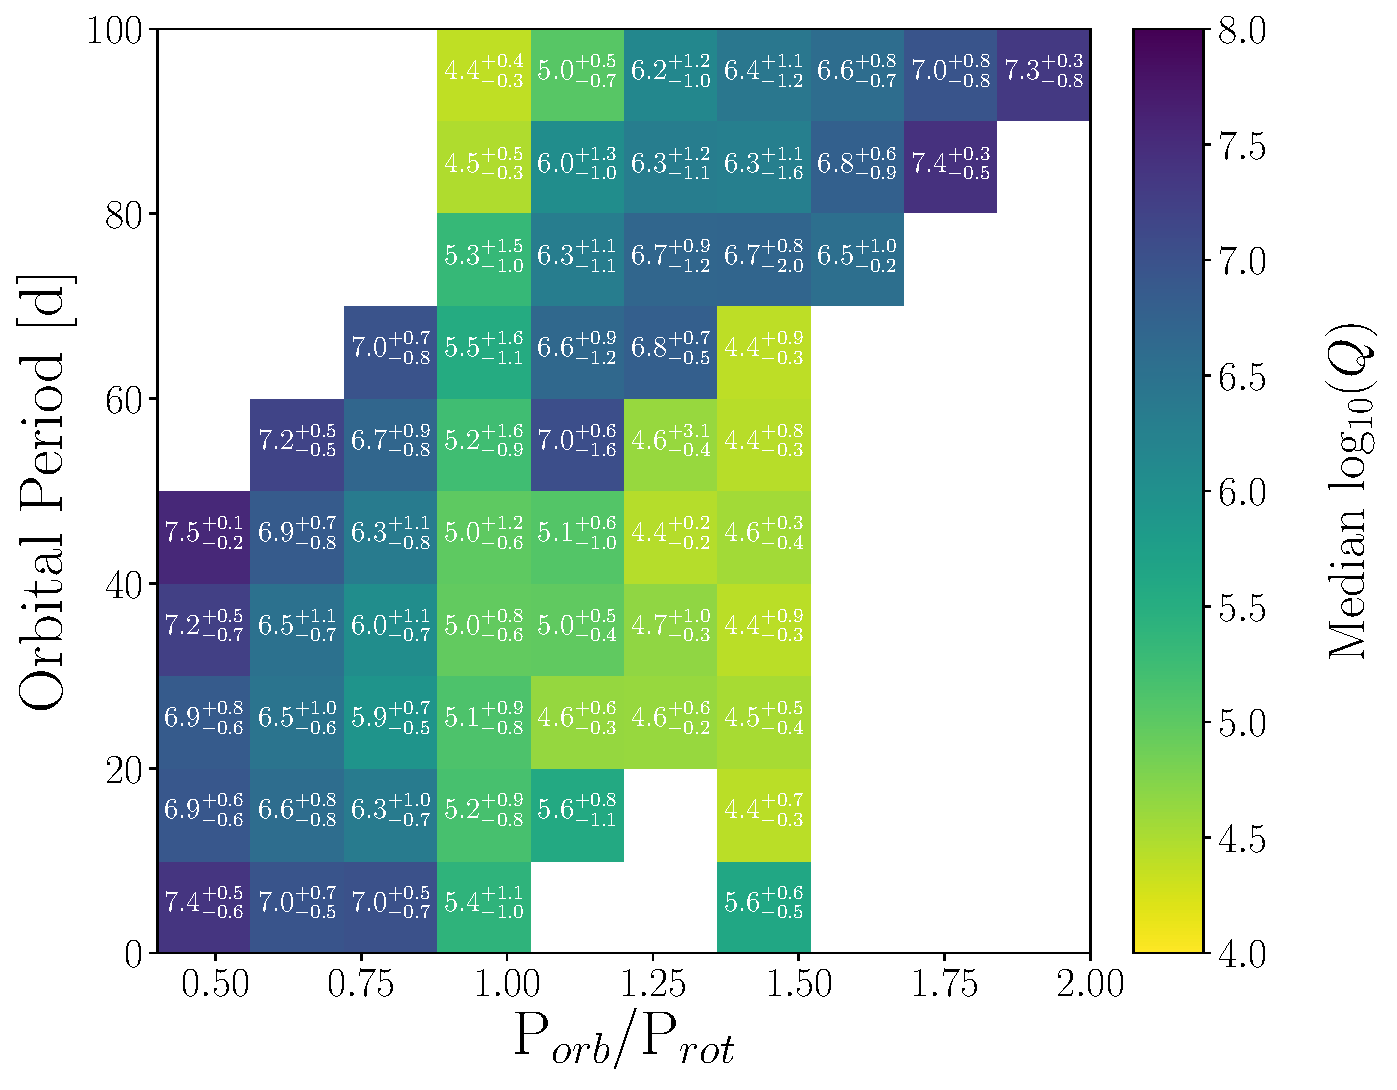
\includegraphics[width=0.45\textwidth]{../Plots/porbProtPorbQHist.pdf}
   \caption{Median log$_{10}(Q)$ of primary stars binned by P$_{orb}$ and P$_{orb}/$P$_{rot}$.  In each bin, we compute the median, $16\%$, and $84\%$ percentiles for log$_{10}(Q)$ and display these values. Narrow constraints imply that certain tidal parameters are required to produce that rotation state, e.g. supersynchronous rotators near P$_{orb}/$P$_{rot} = 1.5$ require $Q \lsim 10^{5.5}$.}%
    \label{fig:qmap}%
\end{figure}

For all P$_{orb}$ in Fig.~\ref{fig:qmap}, synchronous and supersynchronous rotators have systematically low $Q$s, typically $Q < 10^6$, as strong tidal torques are required to tidally-lock the systems, especially for P$_{orb} > 20$ d. For P$_{orb} < 10$ d, there are no rotators with $1.0 <$ P$_{orb}/$P$_{rot} < 1.5$ as strong tidal torques always tidally-lock the binaries.  In this case, P$_{eq}$ can only take two discrete values under the CPL model, i.e. Eqn.~(\ref{eqn:cpl:eqPer}). No stars have P$_{orb}/$P$_{rot} > 1.5$ for P$_{orb} < 70$ d as in the CPL model, binaries with eccentric orbits can only tidally-lock into a 1:1 or 3:2 spin-orbit commensurability.   

Subsynchronous rotators have systematically larger $Q$s, typically $Q > 10^6$, and hence experience weak tidal torques that are dominated by magnetic braking that spin-down the stars past the tidally-locked state.  This effect can be seen for P$_{orb} < 50$ d where the median $Q$ gradually increases with decreasing P$_{orb}/$P$_{rot}$, except near the tidally-locked state that require low $Q$.  This trend reverses at longer P$_{orb} > 60$ d where supersynchronous rotation arises from the inability of tidal torques and magnetic braking to spin-down stars enough to approach the tidally-locked state by the end of the simulation.  In this case, the more supersynchronous the rotation, the weaker the tidal torques must be, and hence the larger the $Q$ must be, as they fail to spin down stars towards P$_{orb}$. 

\begin{figure}
	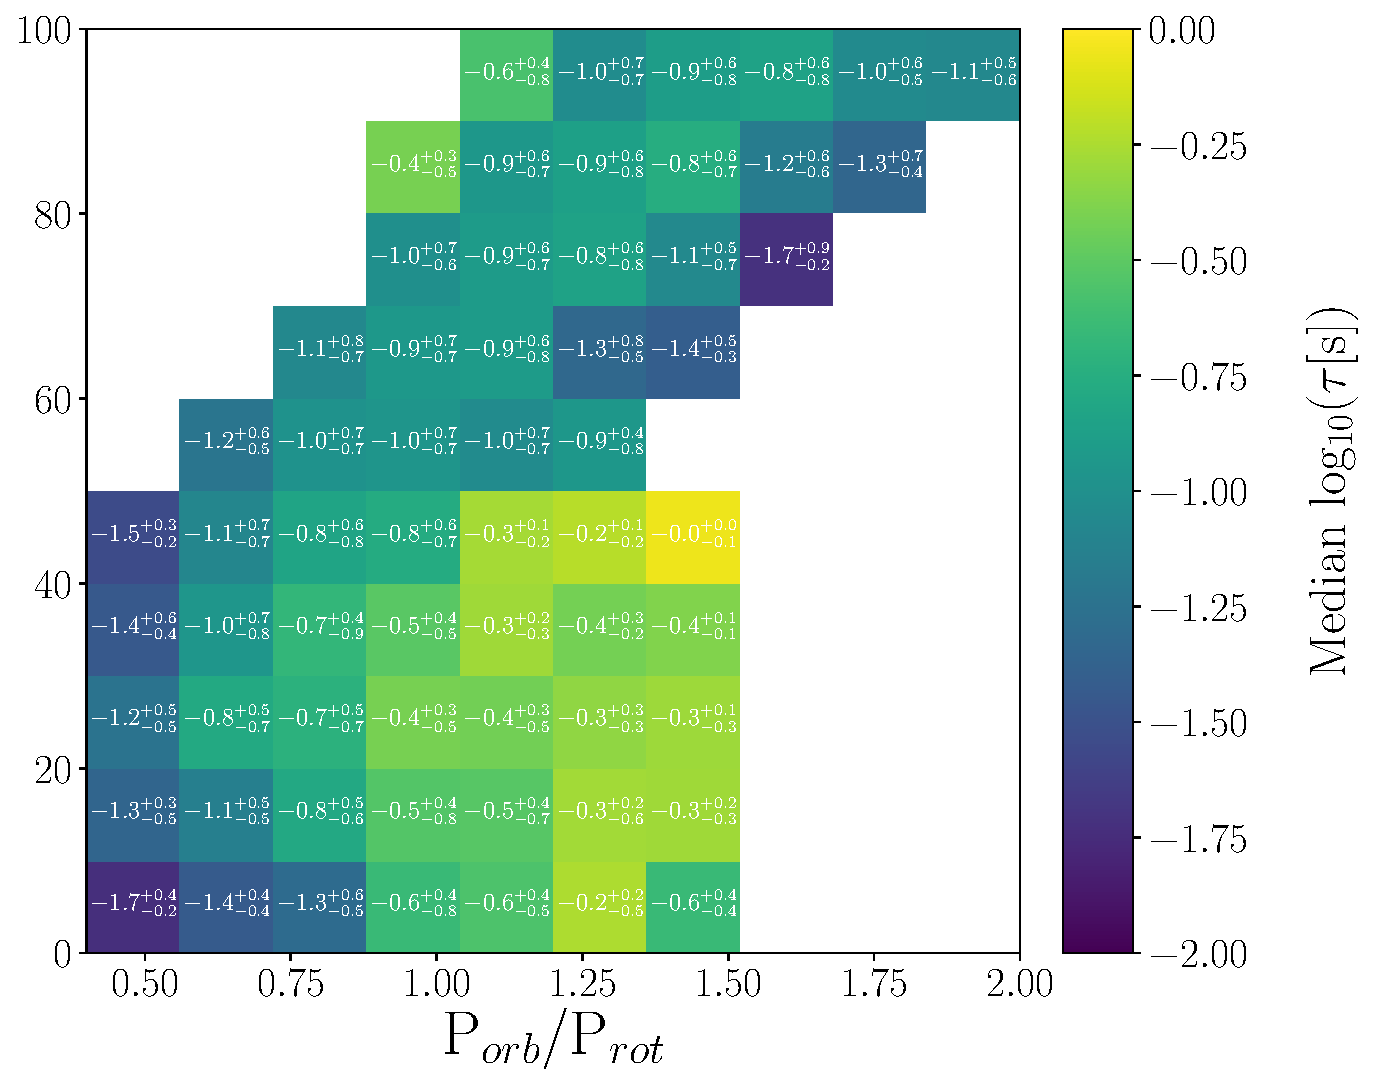
\includegraphics[width=0.45\textwidth]{../Plots/porbProtPorbTauHist.pdf}
   \caption{Same format as Fig.~\ref{fig:qmap}, but for log$_{10}(\tau [s])$ under the CTL model. }%
    \label{fig:taumap}%
\end{figure}

As under the CPL model, stars tidally-lock when subject to strong tidal torques, typically for P$_{orb} < 50$ d and $\tau \gsim 0.25$ s.  For P$_{orb} < 50$ d, subsynchronous rotation occurs for stars with $tau < 0.1$ s as magnetic braking dominates over tidal torques, spinning down the star.  For P$_{orb} > 50$ d, magnetic braking dominates the evolution as the diagonal sequence with a median $\tau \approx 0.1$ s has upper and lower limits that encompass most of the range we considered for $\tau$, suggesting that tides are not important in this region of parameter space.  The shape of this diagonal region arises from the combination of magnetic braking and our flat initial P$_{orb}$ distribution. We do not observe P$_{orb}/$P$_{rot} \gsim 1.5$ as we only consider eccentricities up to $e = 0.3$, limiting how rapid supersynchronous systems can rotate according to Eqn.~(\ref{eqn:ctl:eqPer}).

%% SECTION: COMPARISON TO KEPLER %%
\subsection{Comparison to \kepler} \label{sec:kepler}

Here we compare our simulation results to P$_{rot}$ measurements of primary stars in stellar binaries by \citet{Lurie2017}.  \citet{Lurie2017} measured 816 rotation periods for \kepler EBs with star spot modulations and visually inspected each light curve to ensure their accuracy. The \citet{Lurie2017} dataset is the largest homogenous set of P$_{rot}$ measurements available for low-mass stellar binaries and represents the state of the art benchmark for studies of tidal interactions in stellar binaries. We compare our results to the P$_{1,min}$ P$_{rot}$ values reported by \citet{Lurie2017} as the authors demonstrated that these values are likely to be close to the equatorial P$_{rot}$ that we track in our simulations.

In Fig.~\ref{fig:lurie7}, we display P$_{orb}/$P$_{rot}$ as a function of P$_{orb}$ for both the CPL and CTL models where each simulation was integrated to an age uniformly sampled over $1-7$ Gyr, consistent with ages of \kepler field stars \citep{Chaplin2014}.

- Consult Lurie's paper for CPL vs CTL (e.g. why not 3:2 population-> use CTL!) and for discussing sunsync population. stars prob not in 3:2 resonance since they likely dont have a fixed solid body shape as I assume, but perhaps in a decoupled core envelope model (bouvier?) envelope could get locked into resonance

- compare results to Lurie section 4.4.2 discussion of dependence with eccentricity \citet{Burkart2014}

- lurie finds that low mass ratio binaries are more likely to be subsync for Porb less than 10 days, makes sense since lower mass secondary means weaker tidal torques

\begin{figure*}[t]
	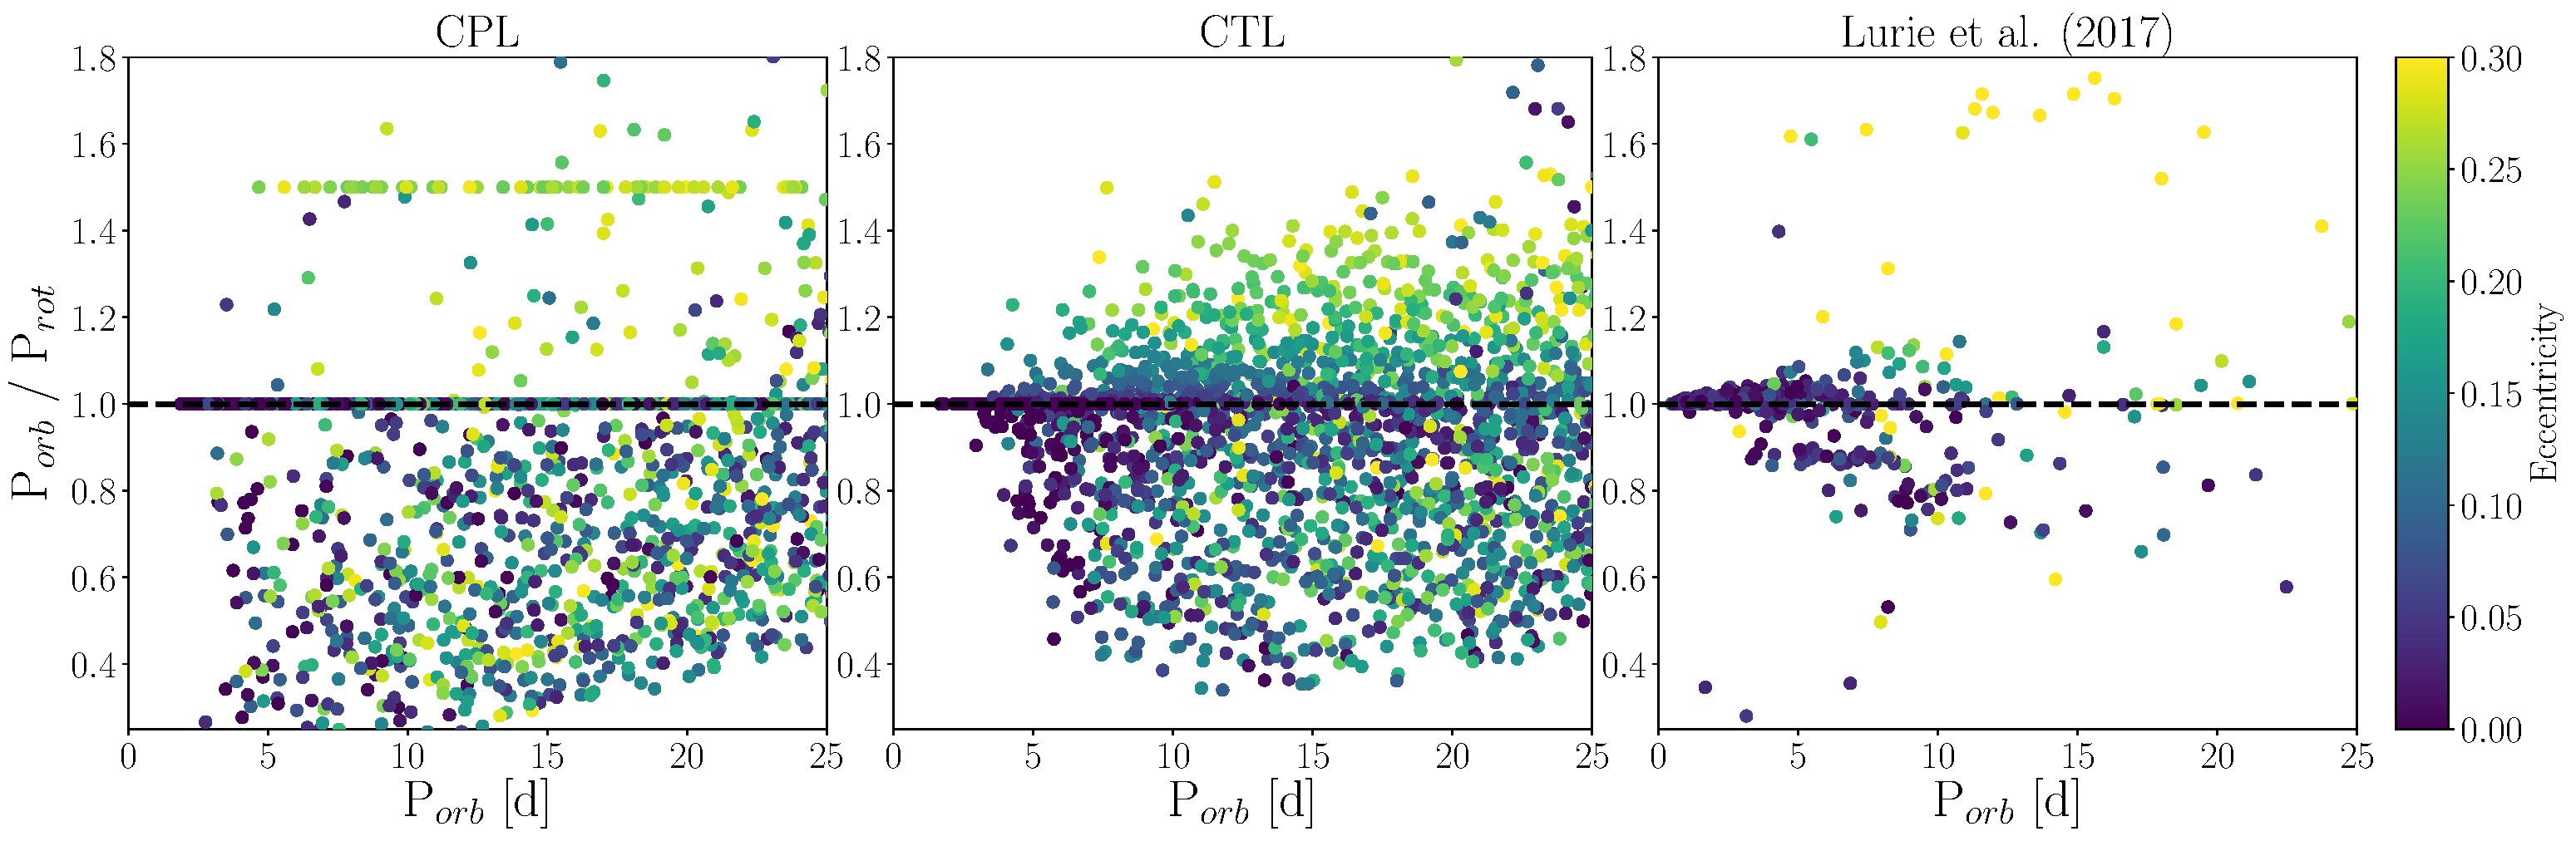
\includegraphics[width=\textwidth]{../Plots/lurieFig7.pdf}
   \caption{P$_{orb}/$P$_{rot}$ as a function of P$_{orb}$ simulated according to the CPL model (left) and the CTL model (right) colored by $e$, compared with \kepler EBs from \citet{Lurie2017} (red plus signs).  The \kepler EBs at low P$_{orb}$ and low P$_{orb}/$P$_{rot}$ are likely either brown dwarfs or exoplanets \citep{Lurie2017}, and hence not modeled by our simulations, so we do not consider them, but we display them for completeness.}%
    \label{fig:lurie7}%
\end{figure*}

XXX

\subsubsection{P$_{orb} < 10$ d: The Subsynchronous Population} \label{sec:subsync}

Median subsync tidal tau: 0.0790922272
Median supersync tidal tau: 0.12508653609999998
Median subsync ecc: 0.1288805
Median supersync ecc: 0.151426
Fraction with Porb/Prot in [0.92,1.2] for Porb < 10d: 0.6126373626373627
Fraction with Porb/Prot in [0.84,0.92] for Porb < 10d: 0.11401098901098901


Although Lurie+2017 attributes differential rotation to the production of the
subsynchronous population, we find that coupled stellar-tidal evolution naturally
produces the population. Compare with Lurie+2017 sample for 2 $<$ Porb $<$ 10 days:
$72\%$ in [0.92,1.2] and $15\%$ in [0.84, 0.92].


\begin{figure}
	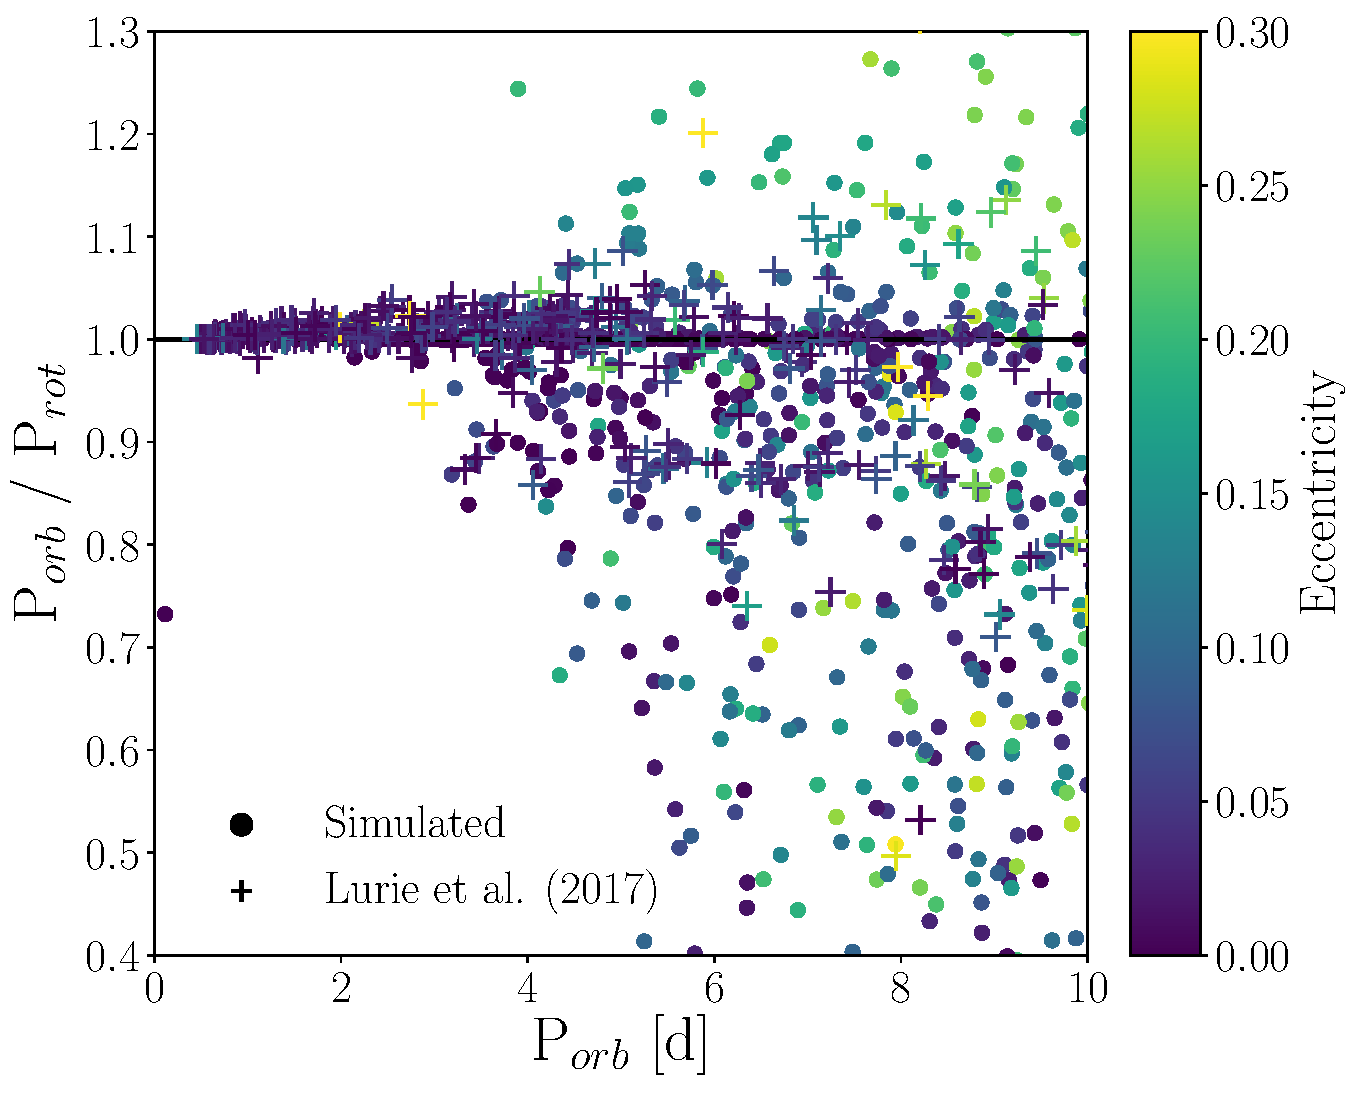
\includegraphics[width=0.45\textwidth]{../Plots/subsync.pdf}
   \caption{Same format as Fig.~\ref{fig:lurie7}, with \citet{Lurie2017} data plotted as diamonds.  All points are colored according to the binary orbital $e$. Our simulations are in excellent agreement with the observed orbital and rotational states of \kepler EBs. }%
    \label{fig:subsync}%
\end{figure}

Our model predicts that nearly all EBs with P$_{orb} < 3$ d are synchronized as is observed by \citet{Lurie2017}. We find that our model predicts a population of supersyncronous rotators on eccentric orbits and a population of subsyncronous rotators with P$_{orb}/$P$_{rot} \approx 0.9$ on nearly-circular orbits, both of which were observed by \citet{Lurie2017}. This excellent agreement between theory and observations validates our model and provides strong evidence that the CTL formalism can accurately model the tidal evolution of low-mass stellar binaries.

\subsubsection{$Q$, $\tau$ Constraints from P$_{orb}$ and P$_{rot}$} \label{sec:qTau}

\begin{figure}
	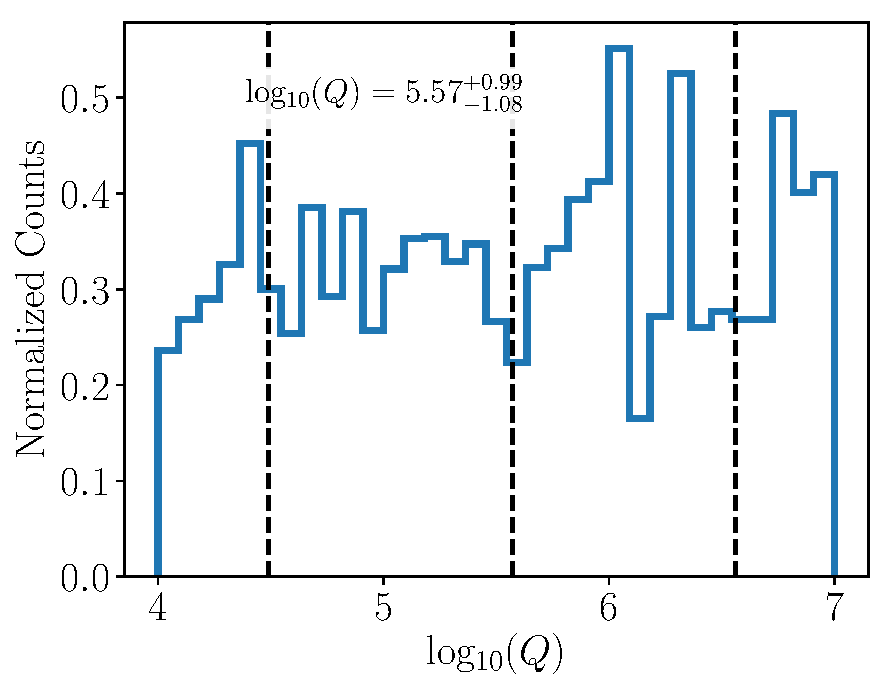
\includegraphics[width=0.45\textwidth]{../Plots/qLurie.pdf}
   \caption{Distribution of stellar tidal $Q$ produced by convolving \citet{Lurie2017} observations of EBs' P$_{rot}$ and P$_{orb}$ with our CPL simulation results shown in Fig.~\ref{fig:qmap}. The dashed black lines, from left to right, indicate the $16^{th}$ percentile, median, and $84^{th}$ percentile. Our $Q$ constraints are consistent with our flat prior distribution over log$_{10}(Q)$, suggesting that tidally-interacting stellar binaries can have a wide range of $Q$.}%
    \label{fig:qLurie}%
\end{figure}

\begin{figure}
	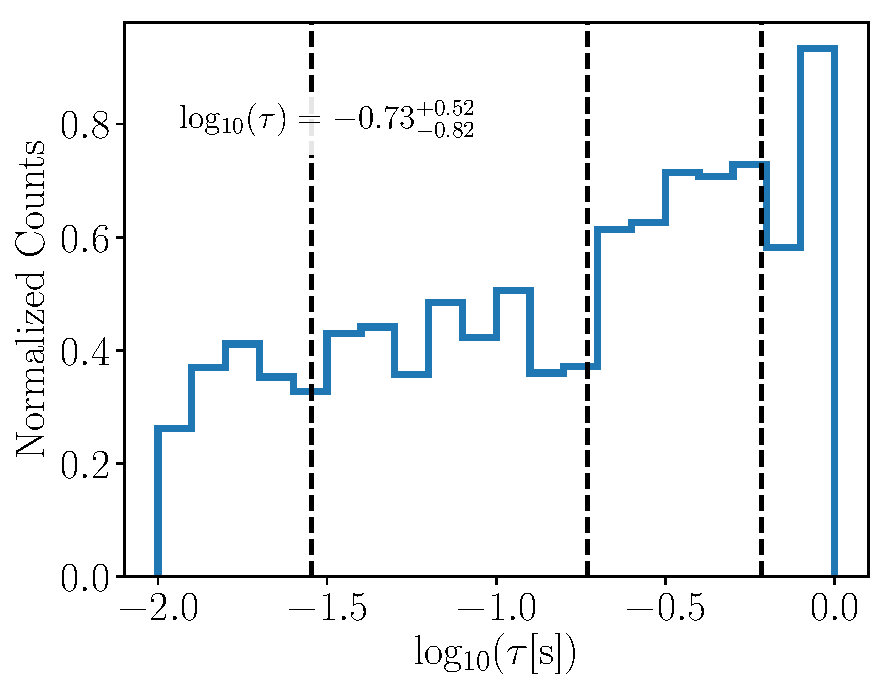
\includegraphics[width=0.45\textwidth]{../Plots/tauLurie.pdf}
   \caption{Same as Fig.~\ref{fig:qLurie}, but using our CTL simulation results from Fig.~\ref{fig:taumap}. We find log$_{10}(\tau) = -0.73^{+0.52}_{-0.82}$ with an increase in density at larger $\tau$ deviating from our prior flat distribution, suggesting that time lags in low-mass stars are larger than the typical value of $\tau \approx 0.1$ s. A wide range of values for $\tau$ are still consistent with observations, however, indicating that tidally-interacting binaries can exhibit a wide range of tidal time lags, albeit with a preference for longer lags.}%
    \label{fig:tauLurie}%
\end{figure}

\subsection{Deviations From Single Star P$_{rot}$ Evolution: Implications for Gyrochronology} \label{sec:gyro}

Here we compare the P$_{rot}$ distribution for tidally-interacting stellar binaries from our CPL and CTL simulations with the P$_{rot}$ distribution of single stars subject to stellar evolution and magnetic braking.  We simulate 10,000 single star systems according to the evolution described in $\S$~\ref{sec:methods:stellar}.  To generate the simulations, we sample from the same mass and initial P$_{rot}$ distributions we used for the binary simulations described $\S$~\ref{sec:methods}. In Fig.~\ref{fig:protDist}, we P$_{rot}$ as a function of mass and age for binaries simulated using both the CPL and CTL model and for single stars. 

Tidally-locked binaries tend to rotate more rapidly than unlocked binaries, reflected in the increased density for P$_{rot} \lsim 20$ d in the marginal distribution for the locked population and in the distribution medians (locked median P$_{rot} = 19.8$ d compared to unlocked median P$_{rot} = 27.5$ d). Binaries readily tidally-lock at short P$_{orb}$ due to the tidal force's strong semi-major axis dependence, increasing the strength of tidal torques at shorter orbital separations. When stellar binaries approach the tidally-locked state, tidal torques overpower the torque due to magnetic braking, fixing P$_{rot} =$ P$_{orb}$, resulting in long-lasting rapid rotation in short P$_{orb}$ binaries. 

Tidal forces modify the spins of unlocked binaries as well, tending to spin-up stars against the effects of magnetic braking towards orbital synchronization, reflected in unlocked binaries' median P$_{rot} = 27.5$ d, compared to the single star median P$_{rot} = 30.6$ d. Tidal locking is not limited to P$_{orb} \lsim 10$ d, however, as we observe stellar binaries to tidally lock out up to P$_{orb} \approx 70$ d, producing a slow-rotating population above the P$_{rot}$ distribution envelop of single stars (compare to XXX). This behavior is consistent with observations of P$_{rot}$ in \kepler eclipsing binaries by \citet{Lurie2017} who find that binaries can tidally lock up to their detection limit of P$_{orb} = $ P$_{rot} = 45$ d. The observed age distribution of tidally-locked binaries has little dependence on P$_{rot}$, with both young and old systems tidally-locking at long and short P$_{rot}$, causing the predictions of gyrochronology models to fail in such systems. 

\begin{figure*}[t]
	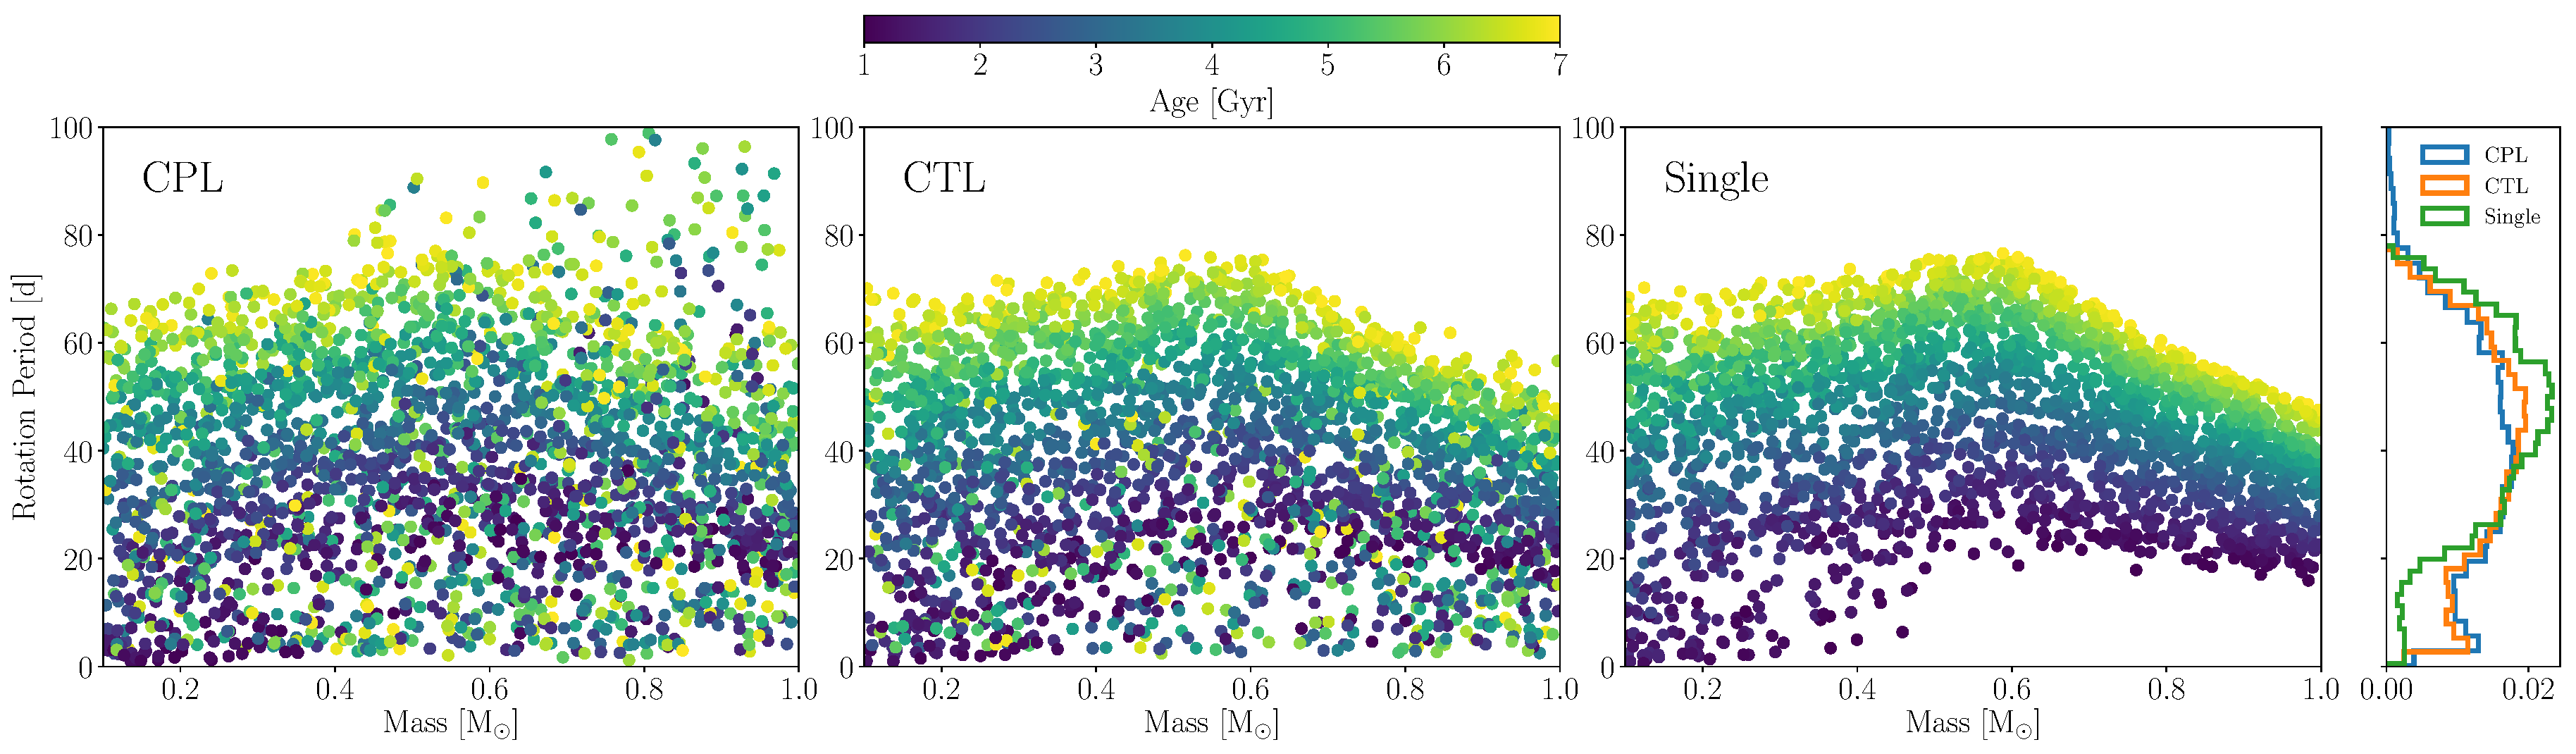
\includegraphics[width=\textwidth]{../Plots/protDist.pdf}
   \caption{P$_{rot}$ as a function of stellar mass and age according to our CPL (left), CTL (left center), and single star (right center) simulations integrated to system ages uniformly sampled over $1-7$ Gyr. The P$_{rot}$ distribution for each case, marginalized over stellar mass, is depicted in the right panel. For each case, we only plot 2,500 systems for clarity but account for all systems when computing the marginalized distributions. Both tidal models predict a substantial population of fast rotators (P$_{rot} < 20$ d) not seen in the single star model at any age, except for young (age $< 2$ Gyr) M dwarfs (M$ < 0.5$ M$_{\odot}$). In many binary systems, both tidal models predict that age does not directly correlate with P$_{rot}$, especially in short P$_{orb}$ binaries where tidal torques are stronger, compared to the clear age-dependence of P$_{rot}$ seen in the single star models, the key assumption of gyrochronology methods. Any application of gyrochonlogy methods to age stars, especially those with P$_{rot} < 20$ d, should rule out or account for binarity.}%
    \label{fig:protDist}%
\end{figure*}

XXX

\begin{figure}
	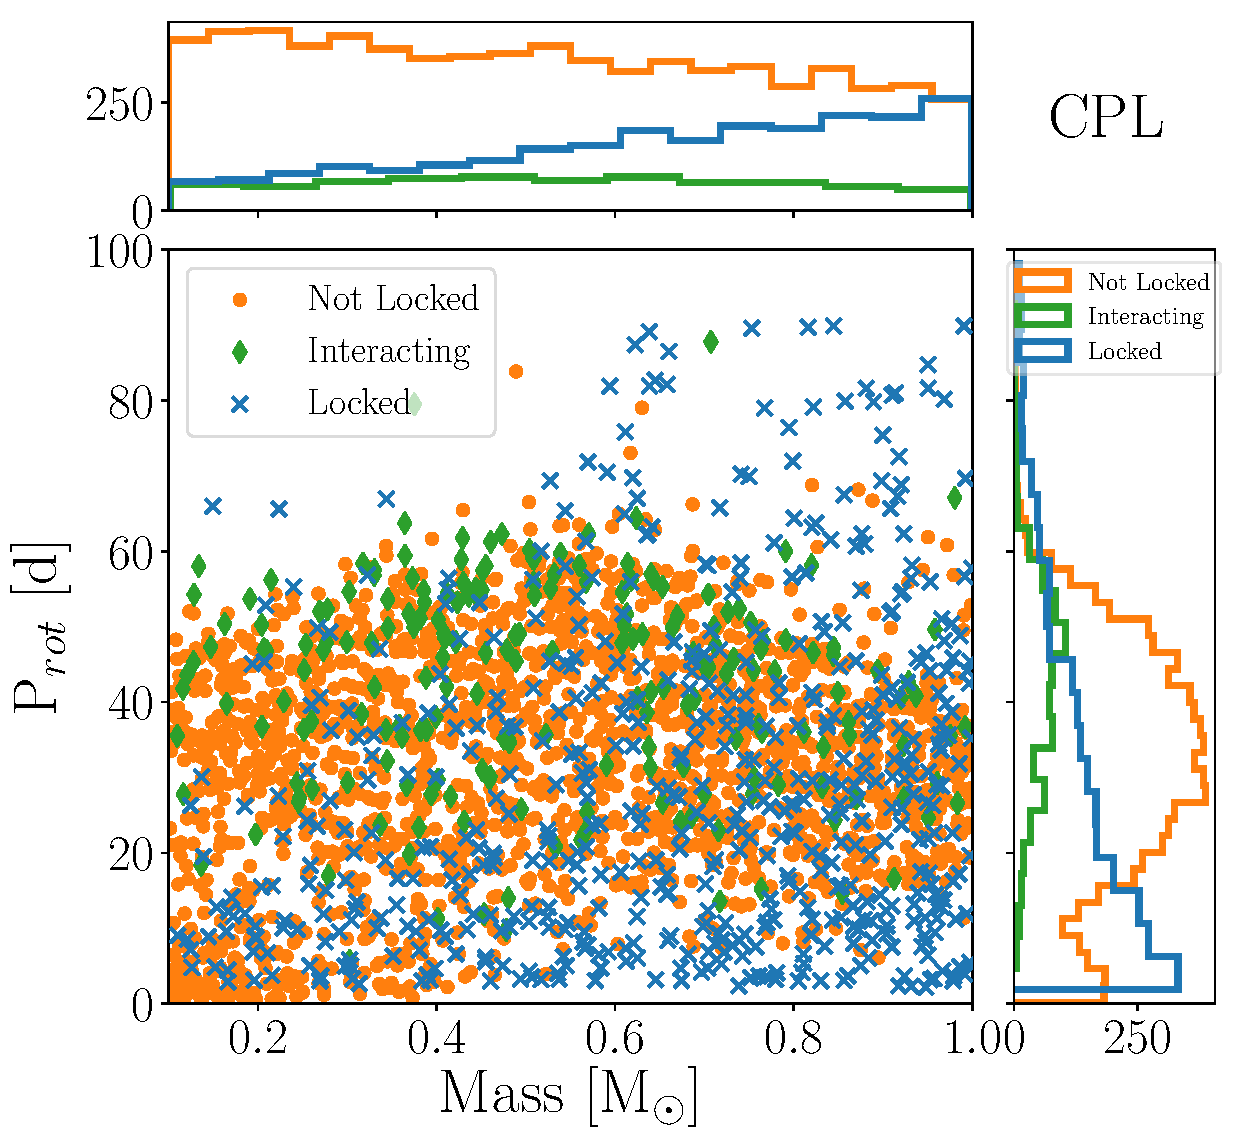
\includegraphics[width=0.45\textwidth]{../Plots/lockedCPL.pdf}
   \caption{Rotation state for tidally-locked (blue, P$_{rot} = $ P$_{eq}$), interacting (green, P$_{rot}$ within $10\%$ of P$_{eq}$ and not locked), and not locked (orange, remainder of binaries) stellar binaries. Left: P$_{rot}$ as a function of stellar mass and age according to our CPL simulations integrated to system ages uniformly sampled over $1-7$ Gyr. Right: P$_{rot}$ distribution for each case, marginalized over stellar mass. Tidally-locked stars systematically rotate faster (median P$_{rot} = 27.0$ d) than interacting (median P$_{rot} = 51.8$ d) and not locked (median P$_{rot} = 41.1$ d) binaries as the locked population typically have shorter P$_{orb}$ where tidal torques are stronger, although binaries up to P$_{orb} = 100$ d tidally-lock. More massive stars are more likely to tidally-lock compared to less massive stars as tidal torques scale with stellar mass, reflected by the enhanced density of locked systems at larger masses. The interacting population tends to rotate more slowly than the unlocked population as at short P$_{orb}$, and hence P$_{rot}$, the systems preferentially tidally-lock.  At longer P$_{orb}$, magnetic braking spin down the stars while tidal torques sheppard P$_{rot}$ towards P$_{eq}$ via the mechanism discussed in $\S$~\ref{sec:eq}. $35\%$ of stars are either tidally-locked or interacting, demonstrating that tidal torques play a pivotal role in shaping the angular momentum evolution in stellar binaries. The P$_{rot}$ - mass distribution for not locked binaries resembles the single star sequence observed in the center right panel of Fig.~\ref{fig:protDist}.}%
    \label{fig:lockedCPL}%
\end{figure}

XXX

\begin{figure}
	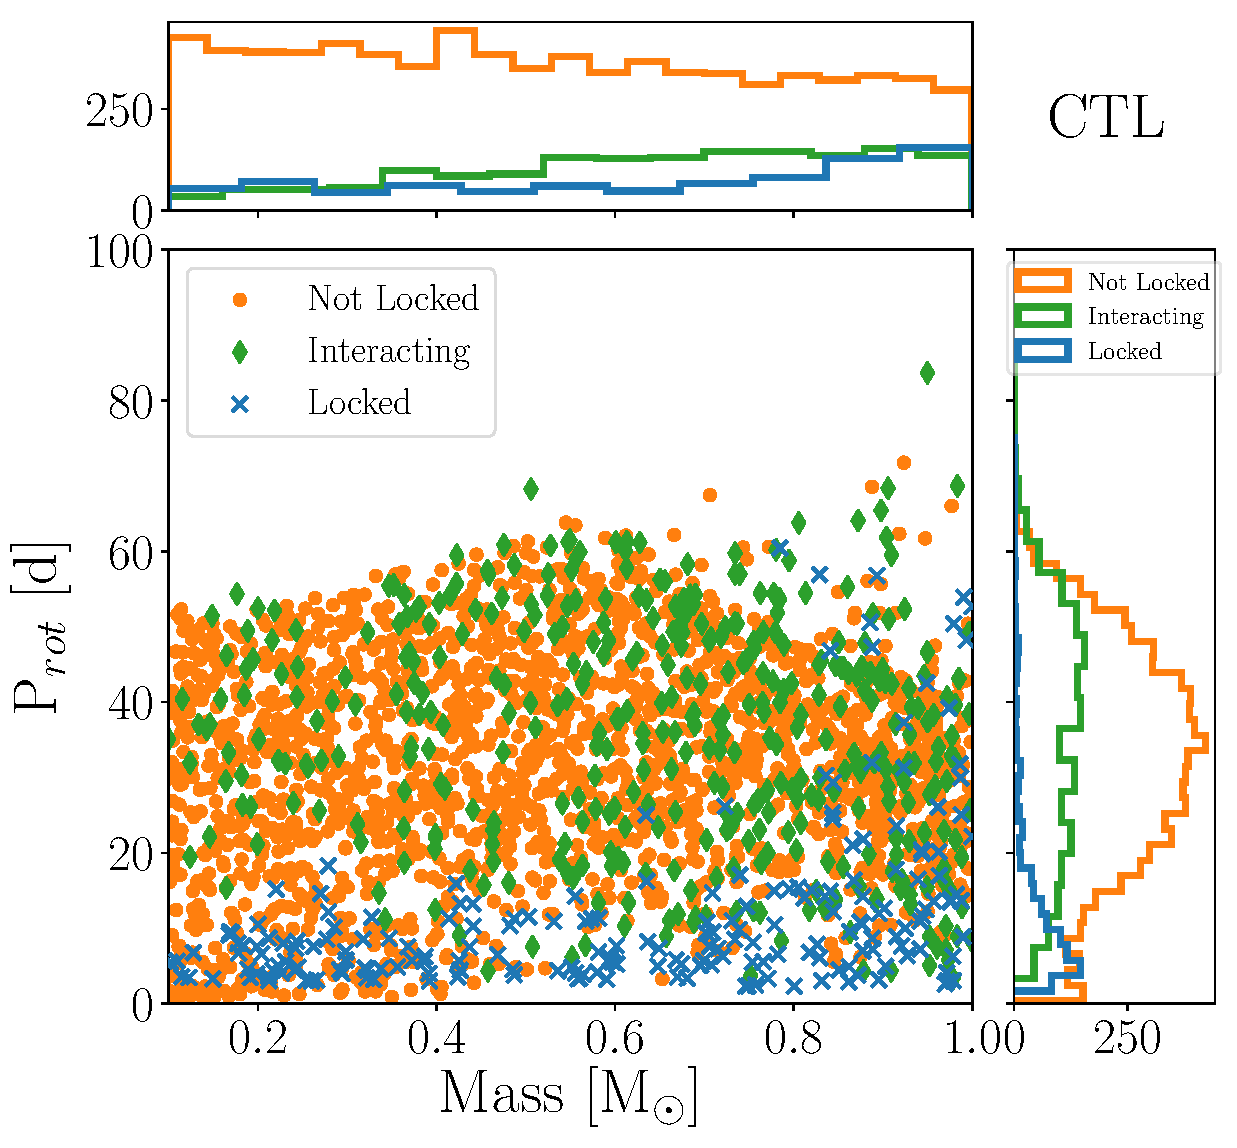
\includegraphics[width=0.45\textwidth]{../Plots/lockedCTL.pdf}
   \caption{Same format as Fig.~\ref{fig:lockedCPL}, but for the CTL simulations. According to the CTL model, only $2\%$ of stellar binaries tidally-locked, mostly at short P$_{orb}$ (median P$_{orb} = 4.8$ d), where tidal torques are strong.  The  $15\%$ of stars are either tidally-locked or interacting, demonstrating that tidal torques play a pivotal role in shaping the angular momentum evolution in stellar binaries. As in Fig.~\ref{fig:lockedCPL}, interacting binaries cluster at longer P$_{rot}$ as magnetic braking overpowers tidal torques to spin down stars, but tidal torques are strong enough to sheppard P$_{rot}$ near P$_{eq}$.}%
    \label{fig:lockedCTL}%
\end{figure}

XXX


\begin{figure}
	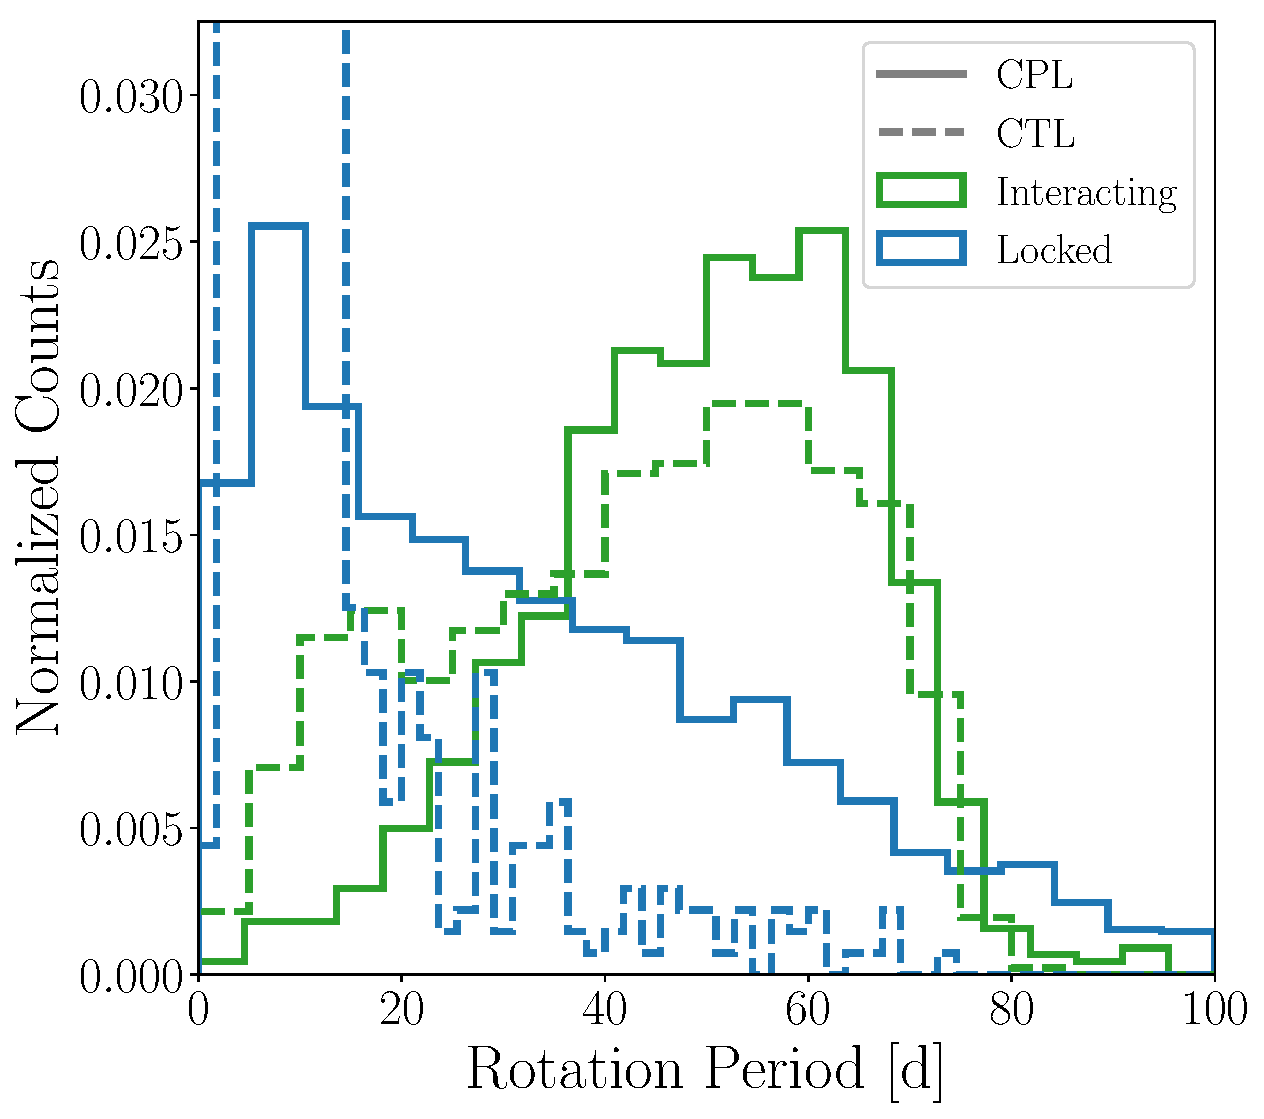
\includegraphics[width=0.45\textwidth]{../Plots/lockedProtHist.pdf}
   \caption{P$_{rot}$ distribution for tidally-locked (blue) and interacting (green, P$_{rot}$ within $10\%$ of P$_{eq}$ and not locked) binaries according to the CPL (solid line) and CTL (dashed line) models. Strong tidal torques in the CPL model can tidally-lock binaries out to P$_{rot} = 100$ d, while weaker torques in the CTL model can only tidally-lock binary stars into a rapid rotation state with P$_{rot} < 20$ d. Under both models, binaries with a wide range of P$_{rot}$ can be strongly tidally-interacting.}%
    \label{fig:lockedProtHist}%
\end{figure}

interacting systems tend to cluster near more massive stars for intermediate periods since their PMS lifetimes are shorter, so they have already spin down and tidal torques are stronger in those systems

%% SECTION: DISCUSSION %%
\section{Discussion} \label{sec:discussion}

XXX

- cite Matsen+2018 for "more than $50\%$ of the binary period distribution will be imaged in about $85\%$ of the host stars" in paper
about detecting unresolved binaries in TESS

- consider dynamical tidal effects (Zahn 1975)?

%% ACKNOWLEDGEMENTS %%
\acknowledgments
This work was facilitated though the use of advanced computational, storage, and networking infrastructure provided by the Hyak supercomputer system and funded by the STF at the University of Washington. This work was supported by NASA Headquarters under the NASA Earth and Space Science Fellowship Program - Grant 80NSSC17K0482.  DPF and RB acknowledge that this work was supported by the NASA Astrobiology Institute's Virtual Planetary Laboratory under Cooperative Agreement number NNA13AA93A. 

%% SOFTWARE %%
%\software{matplotlib: \citet{Hunter2007}, numpy: \citet{vanderWalt2011}, pandas: \citet{Mckinney2010}}

%% BIBLIOGRAPHY %%
\bibliography{sync}

\end{document}

%% End document %%
